\documentclass[letterpaper,12pt]{article}
\usepackage[utf8]{inputenc}
\pagestyle{plain}
\usepackage{graphicx}
\usepackage[small]{caption}
\usepackage{cite}
\usepackage{amsmath}
\usepackage{multirow}
\usepackage{setspace}
\usepackage{xcolor}
\usepackage{authblk}
\usepackage{url}
\usepackage{hyperref}
\usepackage[dvipsnames]{xcolor}

\pagenumbering{roman}

\title{Study of Exclusive $\pi^{0}$ Production Measurement at ePIC of the Future Electron-Ion Collider}
\author[1]{Jihee Kim}

\affil[1]{Department of Physics, Brookhaven National Laboratory, Upton, NY 11973, U.S.A.}

\date{\today}

\begin{document}

\maketitle
\begin{abstract}
The Electron-Ion Collider (EIC) is a next-generation experimental facility designed to investigate the fundamental structure of matter through Deep Inelastic Scattering. Its primary goal is to explore the properties of quarks and gluons in nucleons and nuclei, thereby advancing our understanding of the building blocks of visible matter in the universe. The EIC community outlined the physics program of the EIC in White Paper, and the demanding detector requirements and potential technologies to deploy at an EIC detector were published in a comprehensive Yellow Report. The general-purpose detector resulting from this effort, ePIC,  is designed to perform a broad physics program. 

A key physics channel accessible at the EIC is hard exclusive $\pi^0$ production, which plays a central role in probing Generalized Parton Distributions. This process provides critical insights into the three-dimensional structure of nucleons and nuclei and offers a unique opportunity to study quark orbital angular momentum—a key component in resolving the origin of nucleon mass, a long-standing question in nuclear physics. Additionally, exclusive $\pi^0$ production can mimic the final state of Deeply Virtual Compton Scattering (DVCS), making it a potential background to DVCS measurements. 

In this analysis note, I present a simulation study of the exclusive process $e + p \rightarrow e' + p' + \pi^0$ using the ePIC detector. I evaluate the differential cross-section with respect to the momentum transfer $t$ between the initial and final-state proton, assess the sensitivity of asymmetry measurements in this channel, and estimate the background contribution to DVCS measurement.
\end{abstract}

\begin{figure}[h]
    \centering
    
\includegraphics[scale=0.5]{Figures/EPIC-logo_black.png}
\end{figure}

%\pagebreak
\tableofcontents

\pagebreak
\pagenumbering{arabic}

\section{Introduction}\label{sec:Intro}
% 3D imaging program of EIC - GPD
A central objective of the EIC physics program is to explore the three-dimensional structure of nucleons and nuclei. This structure can be accessed through Generalized Parton Distributions (GPDs), which are experimentally probed via exclusive processes such as Deeply Virtual Compton Scattering (DVCS) and Deeply Virtual Meson Production (DVMP). DVCS offers the cleanest access to GPDs and is particularly sensitive to chiral-even GPDs through its cross-section. In parallel, hard exclusive $\pi^0$ production (DV$\pi^{0}$P), illustrated in Fig.~\ref{fig:dvpi0p}, plays a complementary role by providing sensitivity to chiral-odd GPDs, which are related to quark transversity distributions. 
%The spatial distribution of quarks and gluons can be inferred from the Fourier transform of the differential cross-section with respect to the momentum transfer, $t$, between the incoming and scattered proton.

% Orbital momentum
Moreover, DV$\pi^{0}$P provides a unique opportunity to investigate quark orbital angular momentum (OAM). A recent theoretical study~\cite{PhysRevLett.133.051901} indicates that single-target spin asymmetries in this channel are sensitive to quark OAM. To date, no direct experimental measurement of quark OAM has been performed. The EIC, with its capability for high proton polarization, provides an ideal environment to explore this process. These measurements are expected to contribute significantly to resolving the origin of nucleon mass—a fundamental and long-standing question in nuclear physics.

% Background to DVCS
While DV$\pi^{0}$P is of strong intrinsic interest, it also constitutes a potential background to DVCS measurements. If one of the decay photons from the $\pi^0$ is not detected—due to limited geometric acceptance, energy thresholds, or detector granularity—the event may be misidentified as a DVCS signal. Therefore, DV$\pi^{0}$P must be thoroughly understood and accurately modeled to control background contributions in DVCS analyses.

Previous studies of DV$\pi^{0}$P have been conducted at fixed-target experiments such as JLab and COMPASS, where the accessible kinematic region is dominated by valence quarks. The EIC, in contrast, will provide high proton polarization and broad phase-space coverage, extending into the low-$x$ and high-$Q^2$ regions, thereby enabling a comprehensive investigation of this process.

\begin{figure}[h]
    \centering
    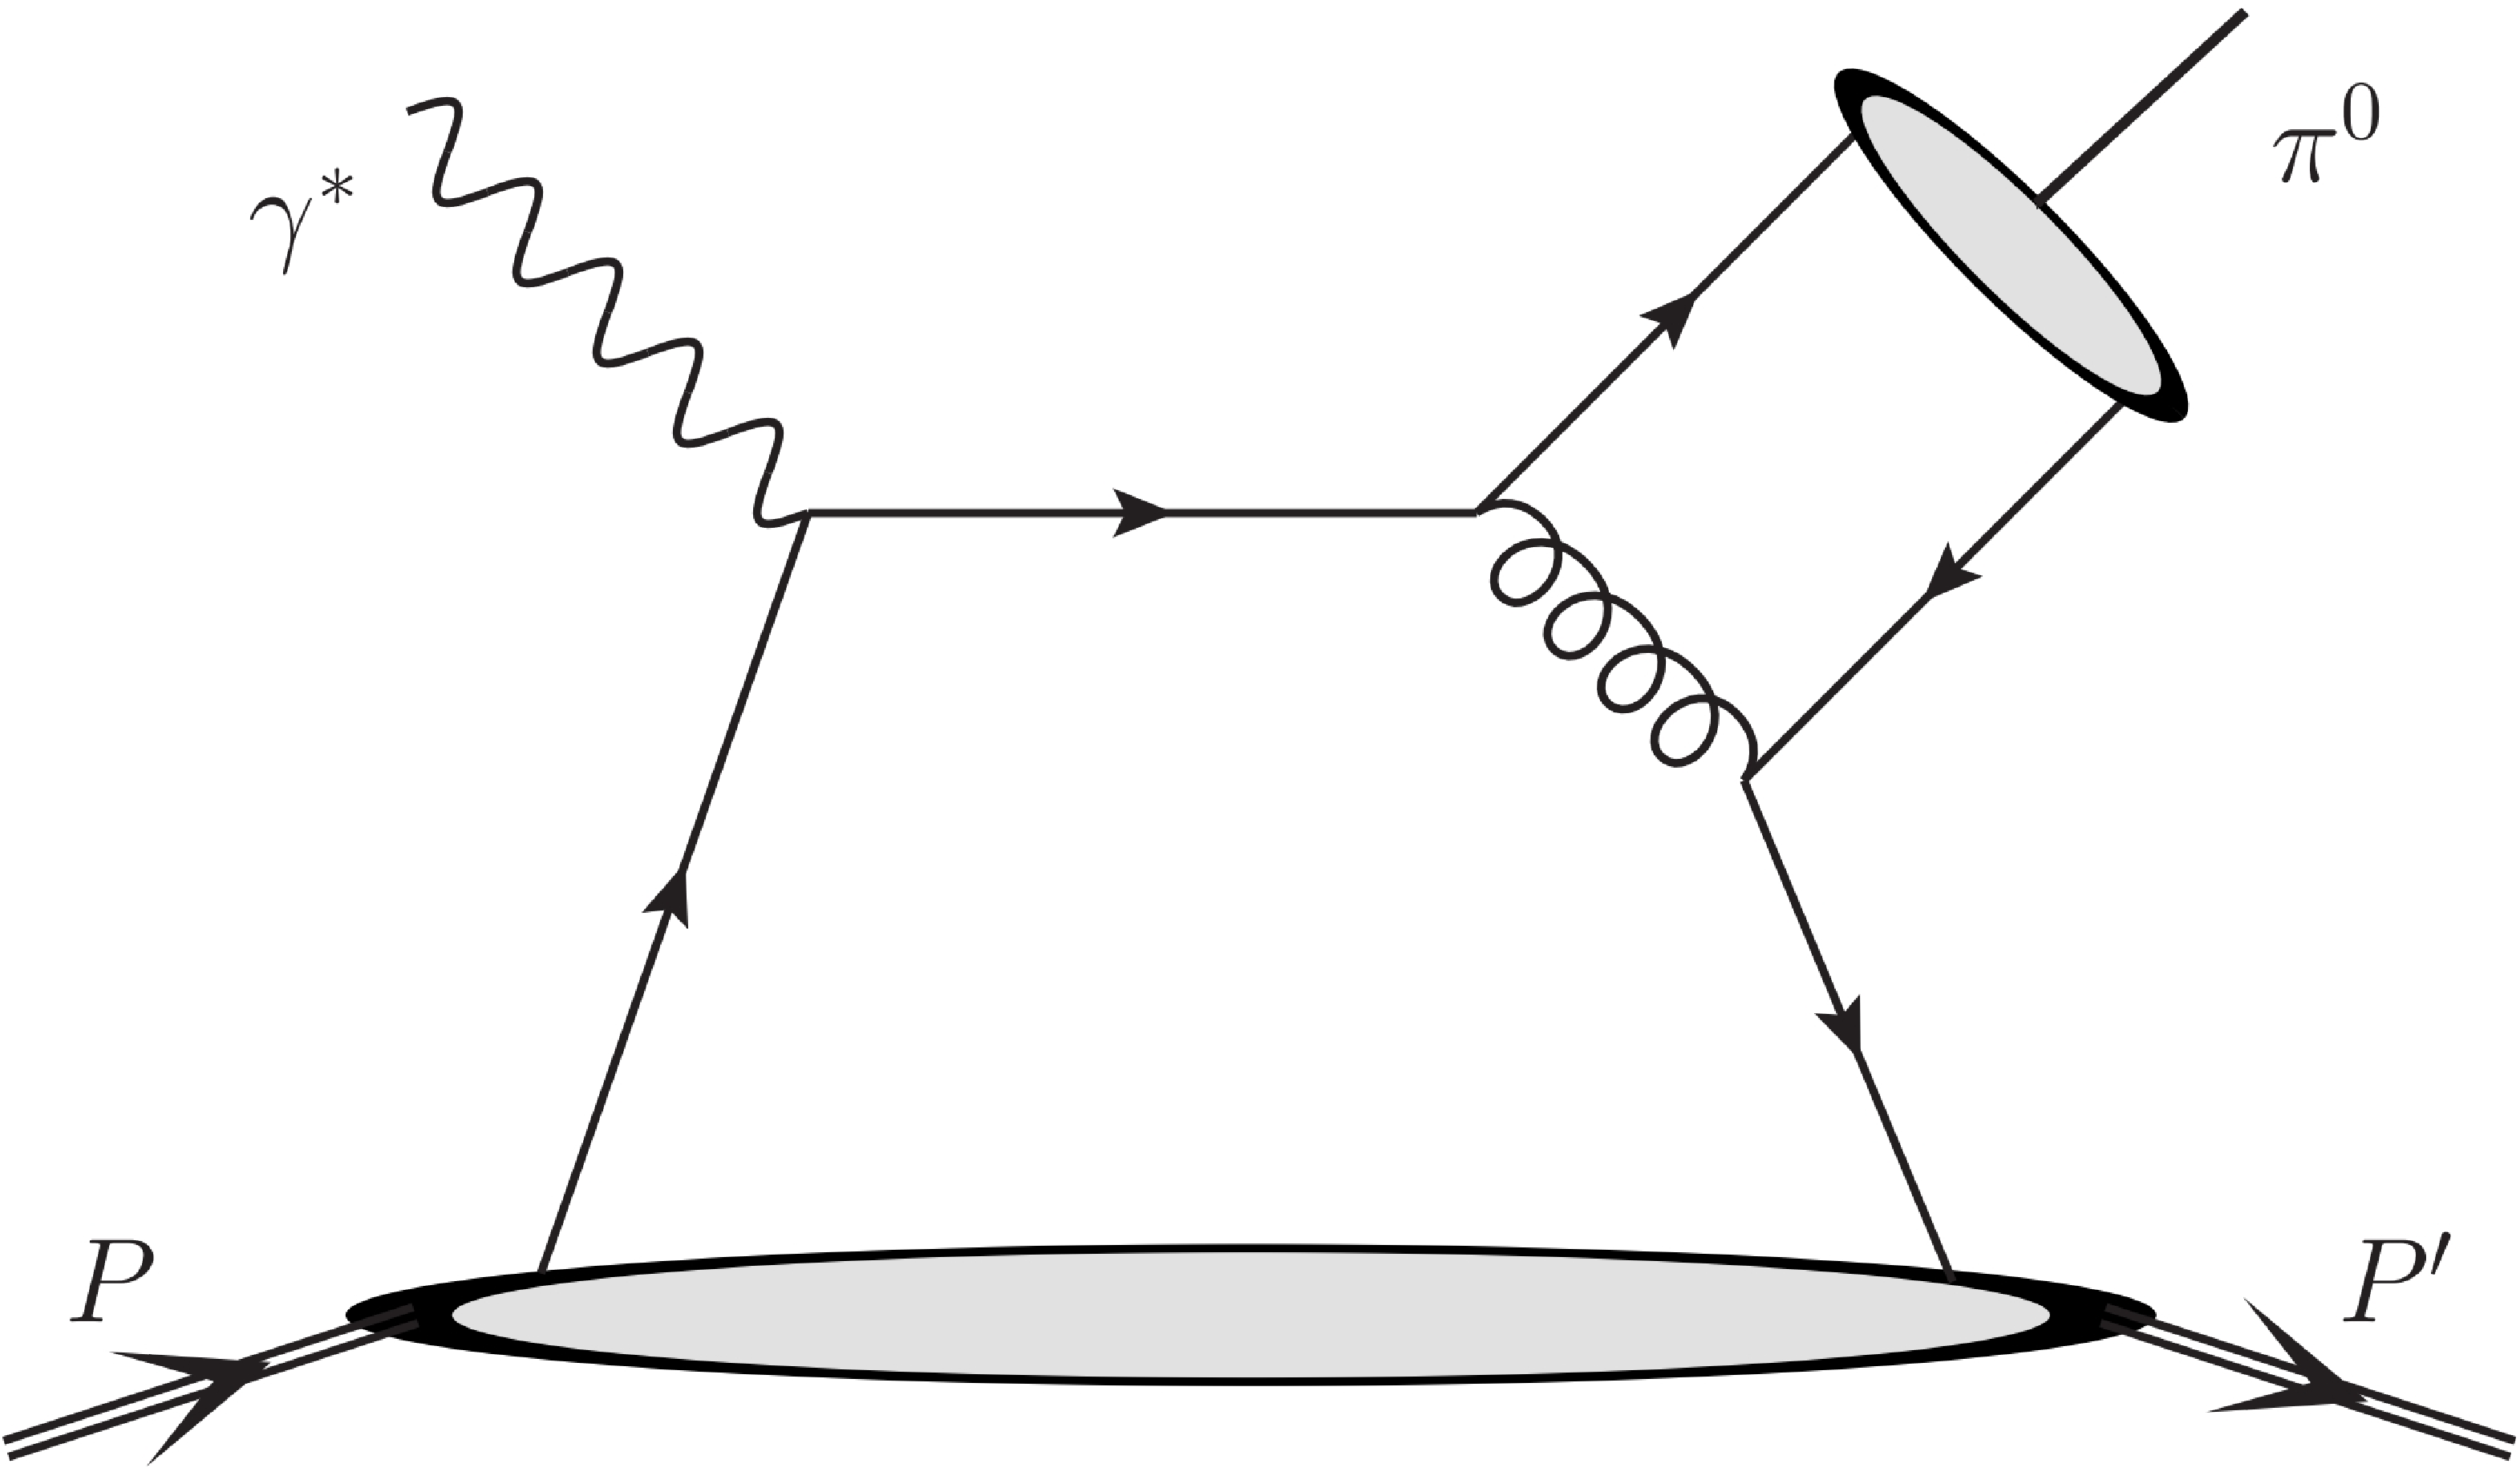
\includegraphics[scale=0.07]{Figures/exclusive_pi0_feynman.pdf}
    \caption{A diagram illustrating the hard exclusive $\pi^0$ production. Taken from \cite{PhysRevLett.133.051901}.}
\label{fig:dvpi0p}
\end{figure}

\section{Simulation Overview}\label{sec:Sim_Overview}
To study the feasibility of the DV$\pi^{0}$P process at the EIC for $ep$ collisions at 10$\times$130 GeV$^2$, exclusive $\pi^{0}$ events ($e + p \rightarrow e' + p' + \pi^0$) were generated privately using the EpIC Monte Carlo generator (version 1.1.6). A total of $1 \times 10^6$ events were processed through the EIC afterburner~\cite{afterburner_github}, which incorporates realistic beam effects such as the crossing angle, angular divergence, and momentum spread. These effects are particularly important for accurate modeling of forward particle acceptance and momentum resolution. The simulated events were then passed through the ePIC detector simulation using the craterlake configuration, followed by reconstruction with the ePIC software framework. The resulting data were used for the final analysis.

\subsection{Event Generator - EpIC}\label{subsec:EvGen}
% EpIC intro
The EpIC\cite{Aschenauer:2022aeb, web_EpIC} is a state-of-the-art Monte Carlo event generator developed for the study of exclusive processes. It is built on the PARTONS platform\cite{Berthou:2015oaw, link_to_PARTONS}, which provides a modular and extensible software architecture, allowing for the integration of a wide range of theoretical models describing the partonic structure of the nucleon. EpIC currently supports a range of exclusive reactions, including Deeply Virtual Compton Scattering (DVCS), Time-like Compton Scattering (TCS), Deeply Virtual Meson Production (DVMP) with $\pi^{0}$, and Double Deeply Virtual Compton Scattering (DDVCS). It also features the implementation of radiative corrections. EpIC is well-suited for both the analysis of existing experimental data and for impact studies, particularly in the context of future experiments at EIC\cite{aschenauer2025studydeeplyvirtualcompton}.

% Generated kinematics
DV$\pi^{0}$P events were generated within the following kinematic ranges:

\begin{itemize}
\item $10^{-5} < x_{B} < 0.95$,
\item $0.01 < y < 0.95$,
\item $1~\text{GeV}^2 < Q^{2} < 1000~\text{GeV}^2$,
\item $0.01~\text{GeV}^2 < |t| < 1.6~\text{GeV}^2$,
\end{itemize}

Fig.~\ref{fig:mcparticle2d} presents the two-dimensional distributions of momentum versus pseudorapidity for the scattered electron, recoil proton, neutral pion, and the two decay photons produced in DV$\pi^{0}$P events from $ep$ collisions.

\begin{figure}[ht]
    \centering
    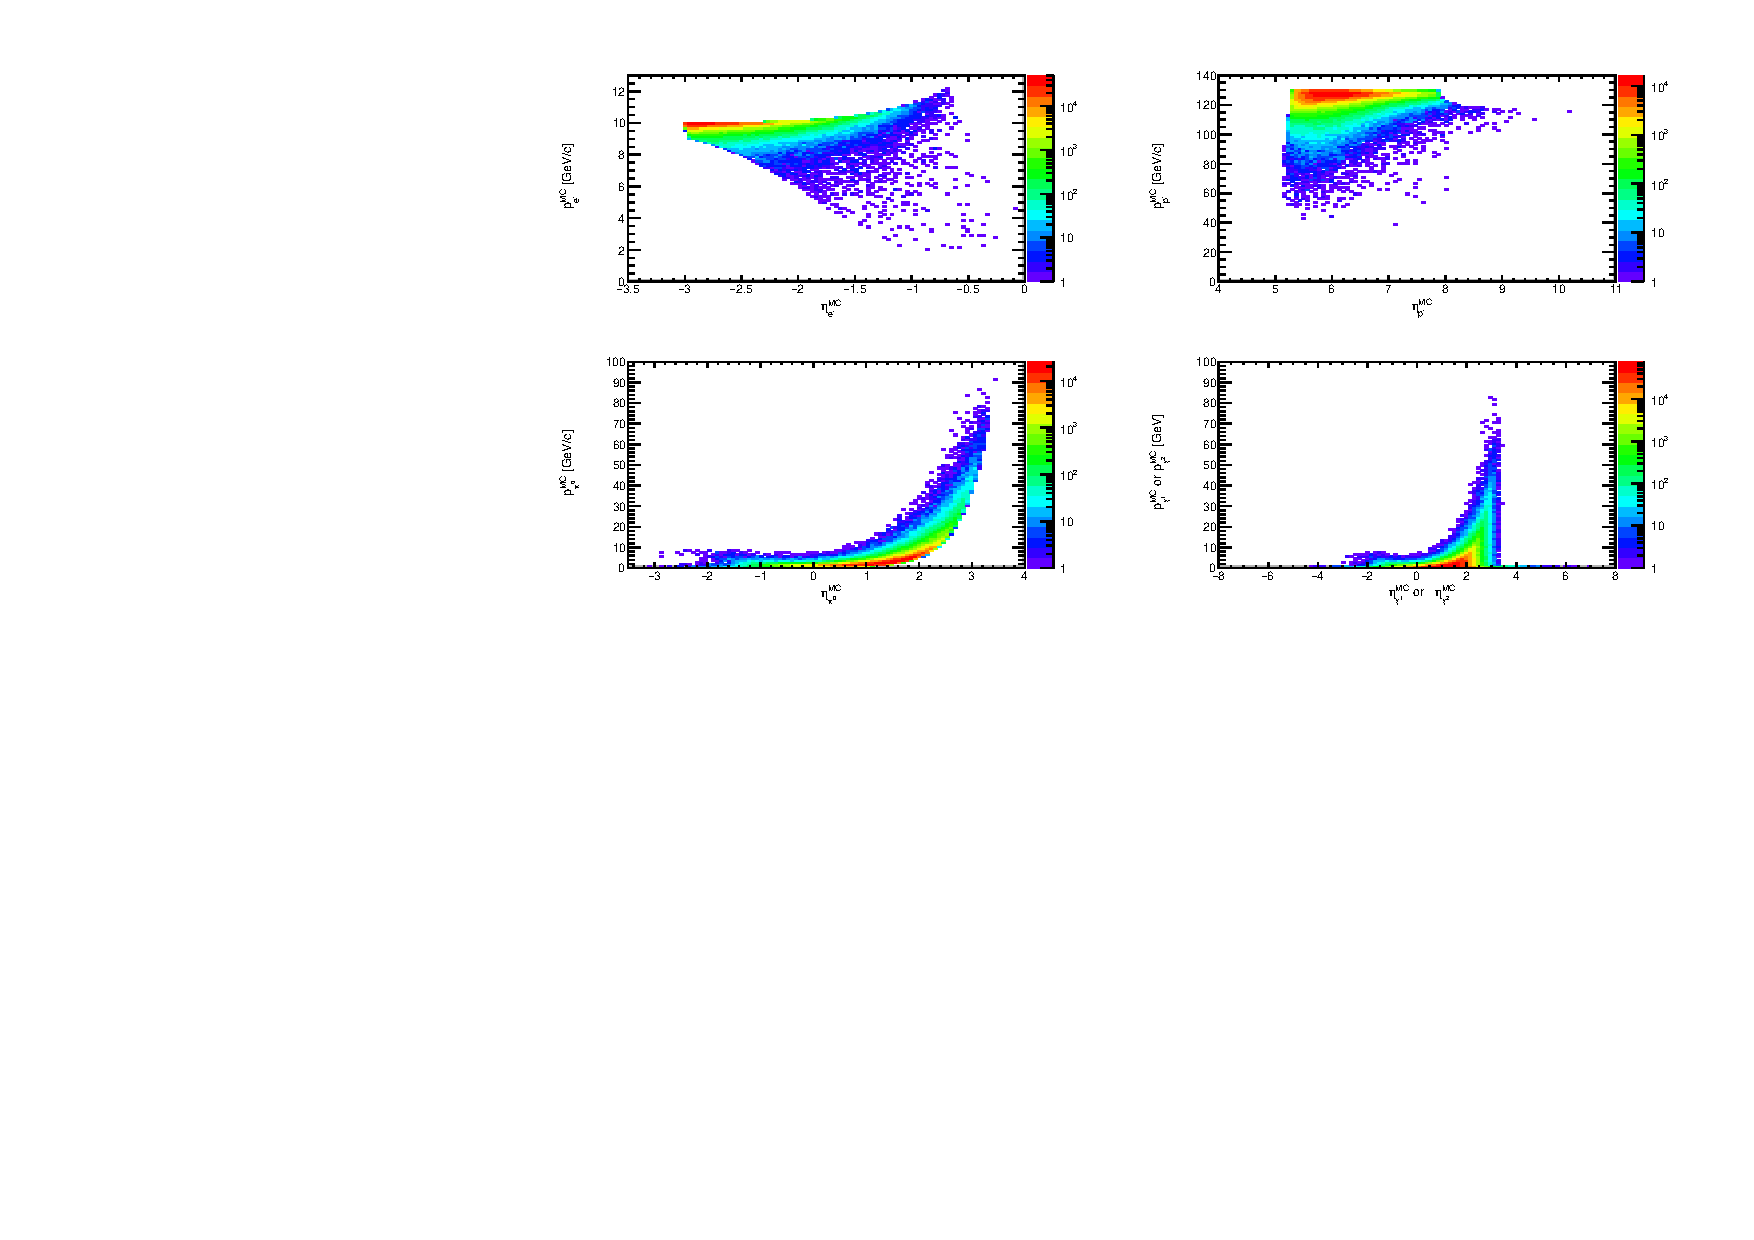
\includegraphics[width=\textwidth]{Figures/MCparticles2D.pdf}
    \caption{The momentum versus pseudorapidity distributions for the scattered electron, recoil proton, neutral pion, and the two decay photons are shown at the generator level.}
\label{fig:mcparticle2d}
\end{figure}

\pagebreak
% How to generate sample
EpIC DV$\pi^0$P events can be generated from the following directory:
\begin{verbatim}
/gpfs/mnt/gpfs02/eic/jkim/run-EpIC-Jihee/
\end{verbatim}

To set up the environment, use:
\begin{verbatim}
source set_env_EpIC
\end{verbatim}

EpIC can then be executed on the RHIC Computing Facility (RCF) using an XML input card. For example:
\begin{verbatim}
run_epic -n 1 -i 10_130_plus_PI0.xml
\end{verbatim}
Here, -n 1 specifies the number of jobs to run, and 10$\_$130$\_$plus$\_$PI0.xml is the configuration file defining the kinematics and process settings for DV$\pi^0$P event generation.

\subsection{Detector Simulation - ePIC}\label{subsec:DetSim}
% EIC afterburner and ePIC detector
DV$\pi^0$P events were processed using the EIC afterburner~\cite{afterburner_github}, which applies realistic beam effects, including the crossing angle, angular divergence, and momentum spread. These effects are essential for accurate modeling of forward particle acceptance and momentum resolution. The afterburned events were subsequently passed through the ePIC detector simulation using the craterlake configuration.

% How to generate Afterburned sample and run ePIC detector simulation
To generate afterburned samples and run detector simulation, the following steps were performed within the eic-shell environment.
Execute the afterburner on the generated HepMC3 DV$\pi^0$P sample using the appropriate beam configuration (ip6$\_$ep$\_$130x10):
\begin{verbatim}
abconv -p ip6_ep_130x10 -o dvpi0p_10_130_plus_1M_ab 
dvpi0p_10_130_plus_1M.hepmc
\end{verbatim}
This produces a new file with beam smearing effects applied.

Still within the eic-shell, set up the detector environment and then run the detector simulation using npsim::
\begin{verbatim}
source /gpfs02/eic/jkim/DVpi0P/epic/install/bin/thisepic.sh

npsim --compactFile ${DETECTOR_PATH}/epic_craterlake_10x130.xml  
--numberOfEvents 10 --filter.tracker ‘edep0’ 
--inputFiles dvpi0p_10_130_plus_1M_ab.hepmc 
--outputFile dvpi0p_10_130_plus_1M_ab.edm4hep.root
\end{verbatim}
This command converts the afterburned events into the EDM4hep format with full detector response simulation applied.

\subsection{Event Reconstruction - ePIC}\label{subsec:EvRecon}
% How to run EICrecon
Event reconstruction was performed within the eic-shell environment using the EICrecon framework. The environment was initialized with:
\begin{verbatim}
source /gpfs02/eic/jkim/DVpi0P/EICrecon/install/bin/eicrecon-this.sh
\end{verbatim}
Once the environment was set, reconstruction was executed with the specific craterlake detector configuration:
\begin{verbatim}
eicrecon -Pdd4hep:xml_files=“${DETECTOR_PATH}”/epic_craterlake_10x130.xml 
-Ppodio:output_file=dvpi0p_10_130_plus_1M_ab.eicrecon.edm4eic.root 
dvpi0p_10_130_plus_1M_ab.edm4hep.root
\end{verbatim}
This command processes the simulated EDM4hep input file and produces a reconstructed output, which is used for subsequent analysis.

\section{Event Selection}\label{sec:EvSelect}
% Intro
For this DV$\pi^0$P study, event exclusivity is required, meaning that all final-state particles must be detected: the scattered electron, the two photons from the $\pi^0$ decay, and the recoil proton. The scattered electron and decay photons are detected within the central detector, while the recoil proton is measured using the far-forward detection systems—specifically, the B0 spectrometer and the Roman Pot (RP) detectors. The following sections describe the detector acceptance and the selection criteria applied to each of these final-state particles.

\subsection{Scattered Electron}\label{subsec:ScatteredElectron}
% Acceptance and quality cut
Accurate identification and reconstruction of the scattered electron are crucial, as they determine the kinematics of the Deep Inelastic Scattering (DIS) event. Electron selection in this study was performed using truth-level association. If a cluster was found in the backward electromagnetic calorimeter (EMCal), the cluster energy was used to reconstruct the electron's four-momentum, while the position (pseudorapidity and azimuthal angle) was taken from the tracker. An $E/p$ cut was applied—defined as the ratio of the cluster energy ($E$) to the track momentum ($p$)—with the requirement that $0.8 < E/p < 1.2$ for an electron to be considered well reconstructed. In events where no backward EMCal cluster was available, the four-momentum of the scattered electron was reconstructed using only tracking information. The left panel of Fig.~\ref{fig:electron} shows the detector acceptance for the scattered electron as a function of pseudo-rapidity, with an overall acceptance of approximately 89.8~\%. The right panel compares the energy distributions of the true, accepted (within detector acceptance), and reconstructed scattered electrons. These results indicate that there may be room for improving the reconstruction and/or refining the quality selection criteria.

Following electron selection, DIS kinematic variables were calculated, shown in Fig.~\ref{fig:diskinematics}. The upper panels compare the distributions of accepted true and reconstructed values for each kinematic variable, while the lower panels show two-dimensional correlations between the true and reconstructed values. Overall, the reconstructed DIS kinematics agree well with the truth-level values, with the exception of the Bjorken-$x$ variable, where larger deviations are observed. This again indicates that further refinement in electron reconstruction and selection criteria could enhance the accuracy of the kinematic reconstruction.

\begin{figure}[ht]
    \centering
    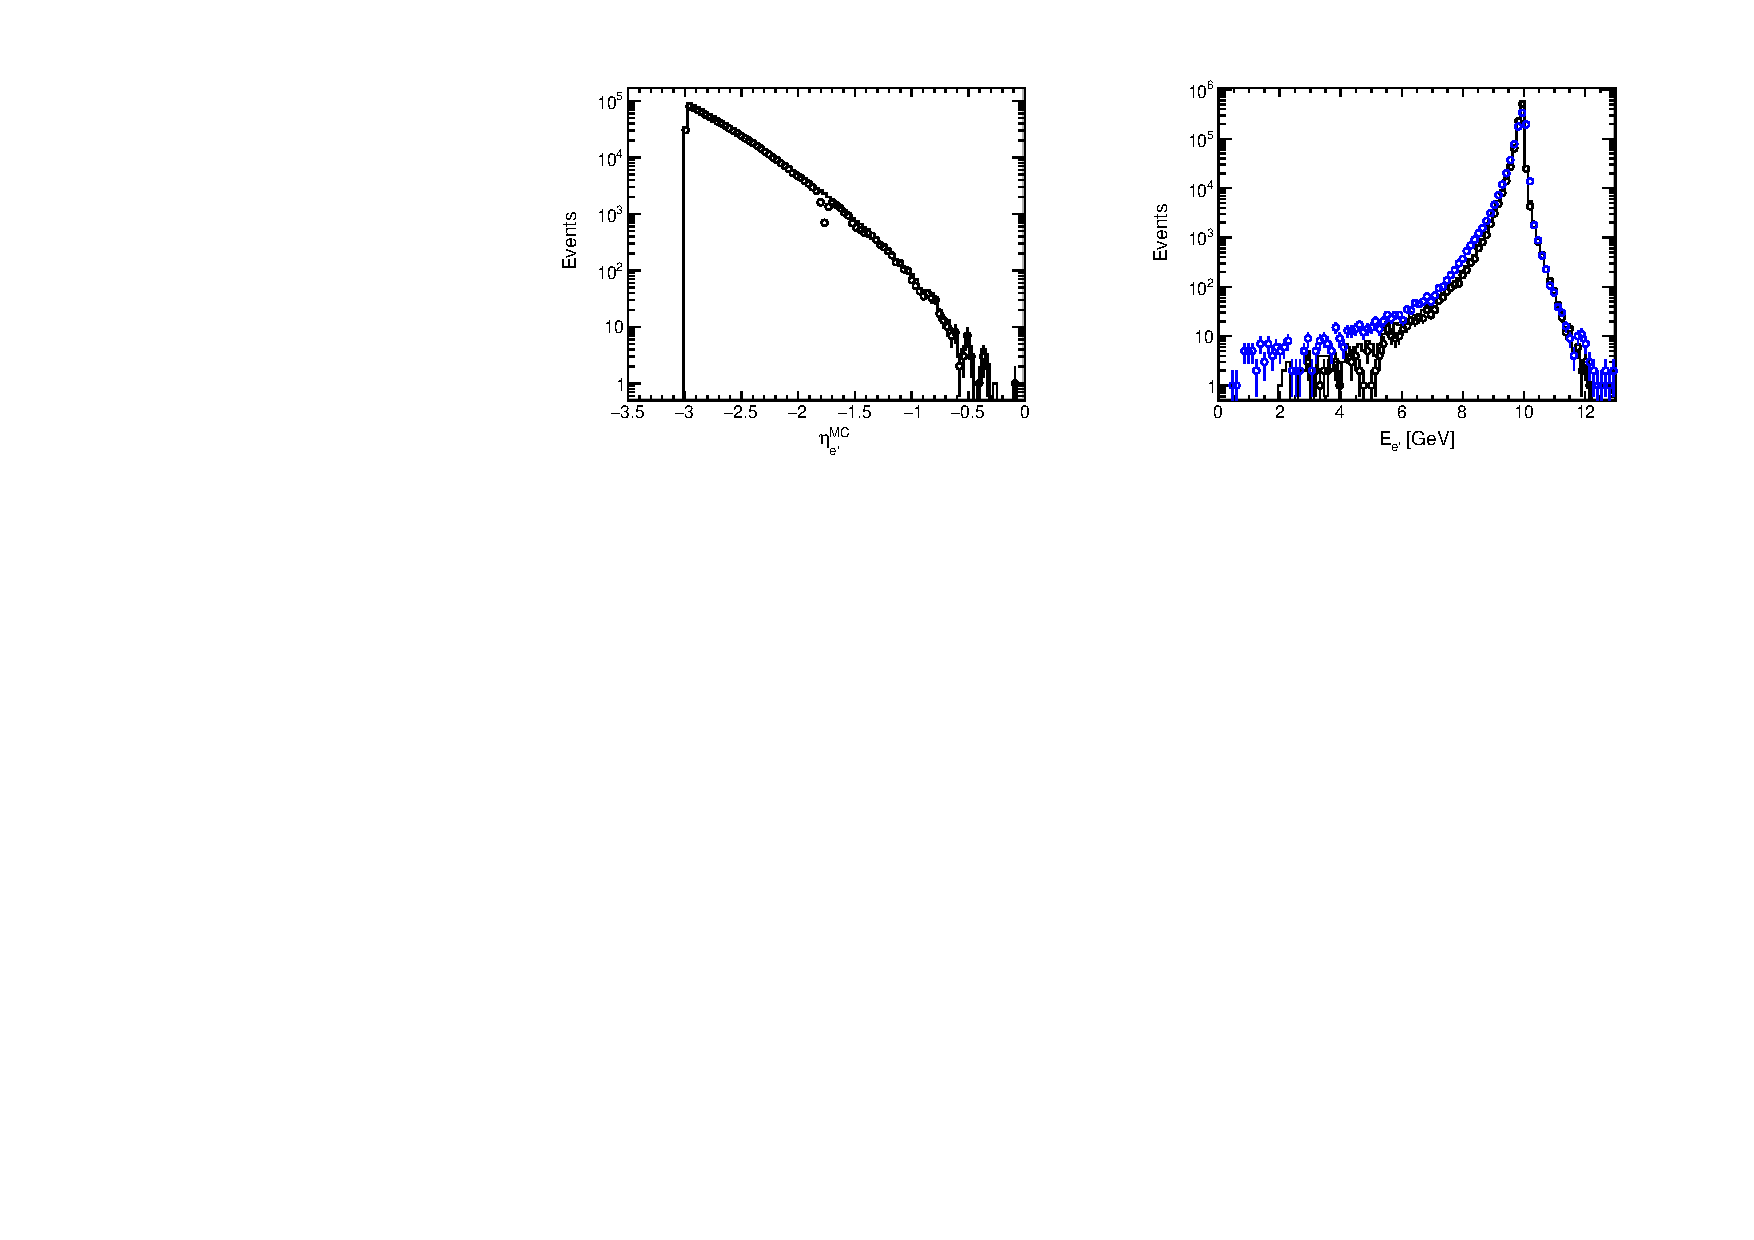
\includegraphics[width=0.75\textwidth]{Figures/electron.pdf}
    \caption{(Left) Detector acceptance for the scattered electron as a function of pseudorapidity. (Right) Energy distributions of the true scattered electron (black solid line), accepted true values within detector acceptance (black open circles), and reconstructed values (blue open circles).}
\label{fig:electron}
\end{figure}

\begin{figure}[h]
    \centering
    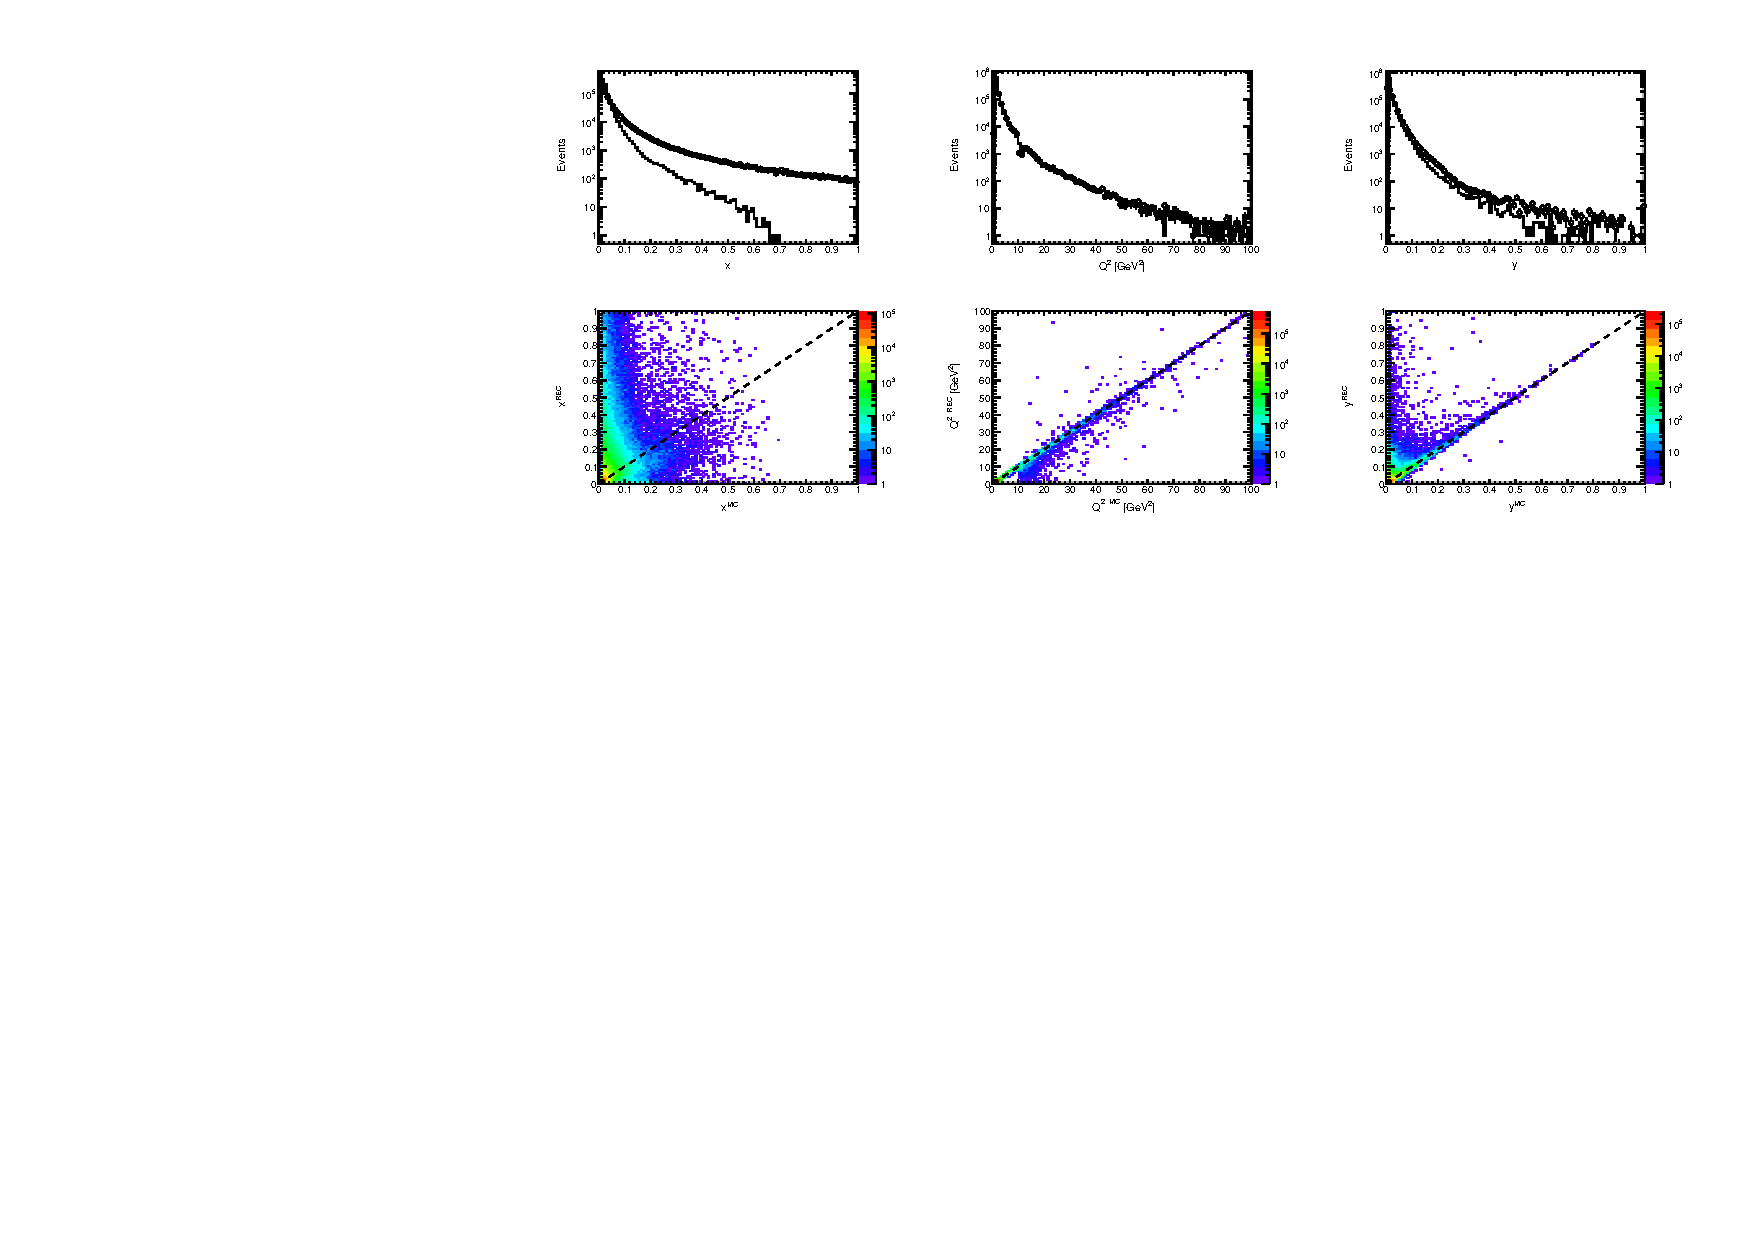
\includegraphics[scale=0.6]{Figures/DIS_kinematics.pdf}
    \caption{Comparison of DIS kinematic variables: $x$, $Q^{2}$, and $y$. (Top row) Distributions of accepted true and reconstructed values for each variable. (Bottom row) Two-dimensional correlations between true and reconstructed values.}
\label{fig:diskinematics}
\end{figure}

\subsection{Scattered Proton}\label{subsec:ScatteredProton}
% Acceptance and quality cut
For events in which the proton is detected in the B0 spectrometer, the \colorbox{lightgray}{ReconstructedTruthSeededChargedParticles} data collection was used. When the proton is detected in the RP detectors, the \colorbox{lightgray}{ForwardRomanPotRecParticles} data collection was employed for reconstruction. The left panel of Fig.~\ref{fig:protonacc} shows the detector acceptance for the scattered proton as a function of pseudo-rapidity, illustrating a gap in acceptance between the B0 and RP detector. The right panel displays the distribution of the squared momentum transfer, $t$, as accepted from the true protons. This distribution also reflects the acceptance gap between the two far-forward detectors. Fig.~\ref{fig:protonrec} shows the reconstructed momentum of the recoil proton and the corresponding $t$ distribution. It should be noted that these results include contributions from poorly reconstructed protons due to the use of static matrix reconstruction, and that no quality cuts have yet been applied. Consequently, there is a potential for improving the scattered proton selection with enhanced reconstruction methods and stricter quality criteria.

\begin{figure}[ht]
    \centering
    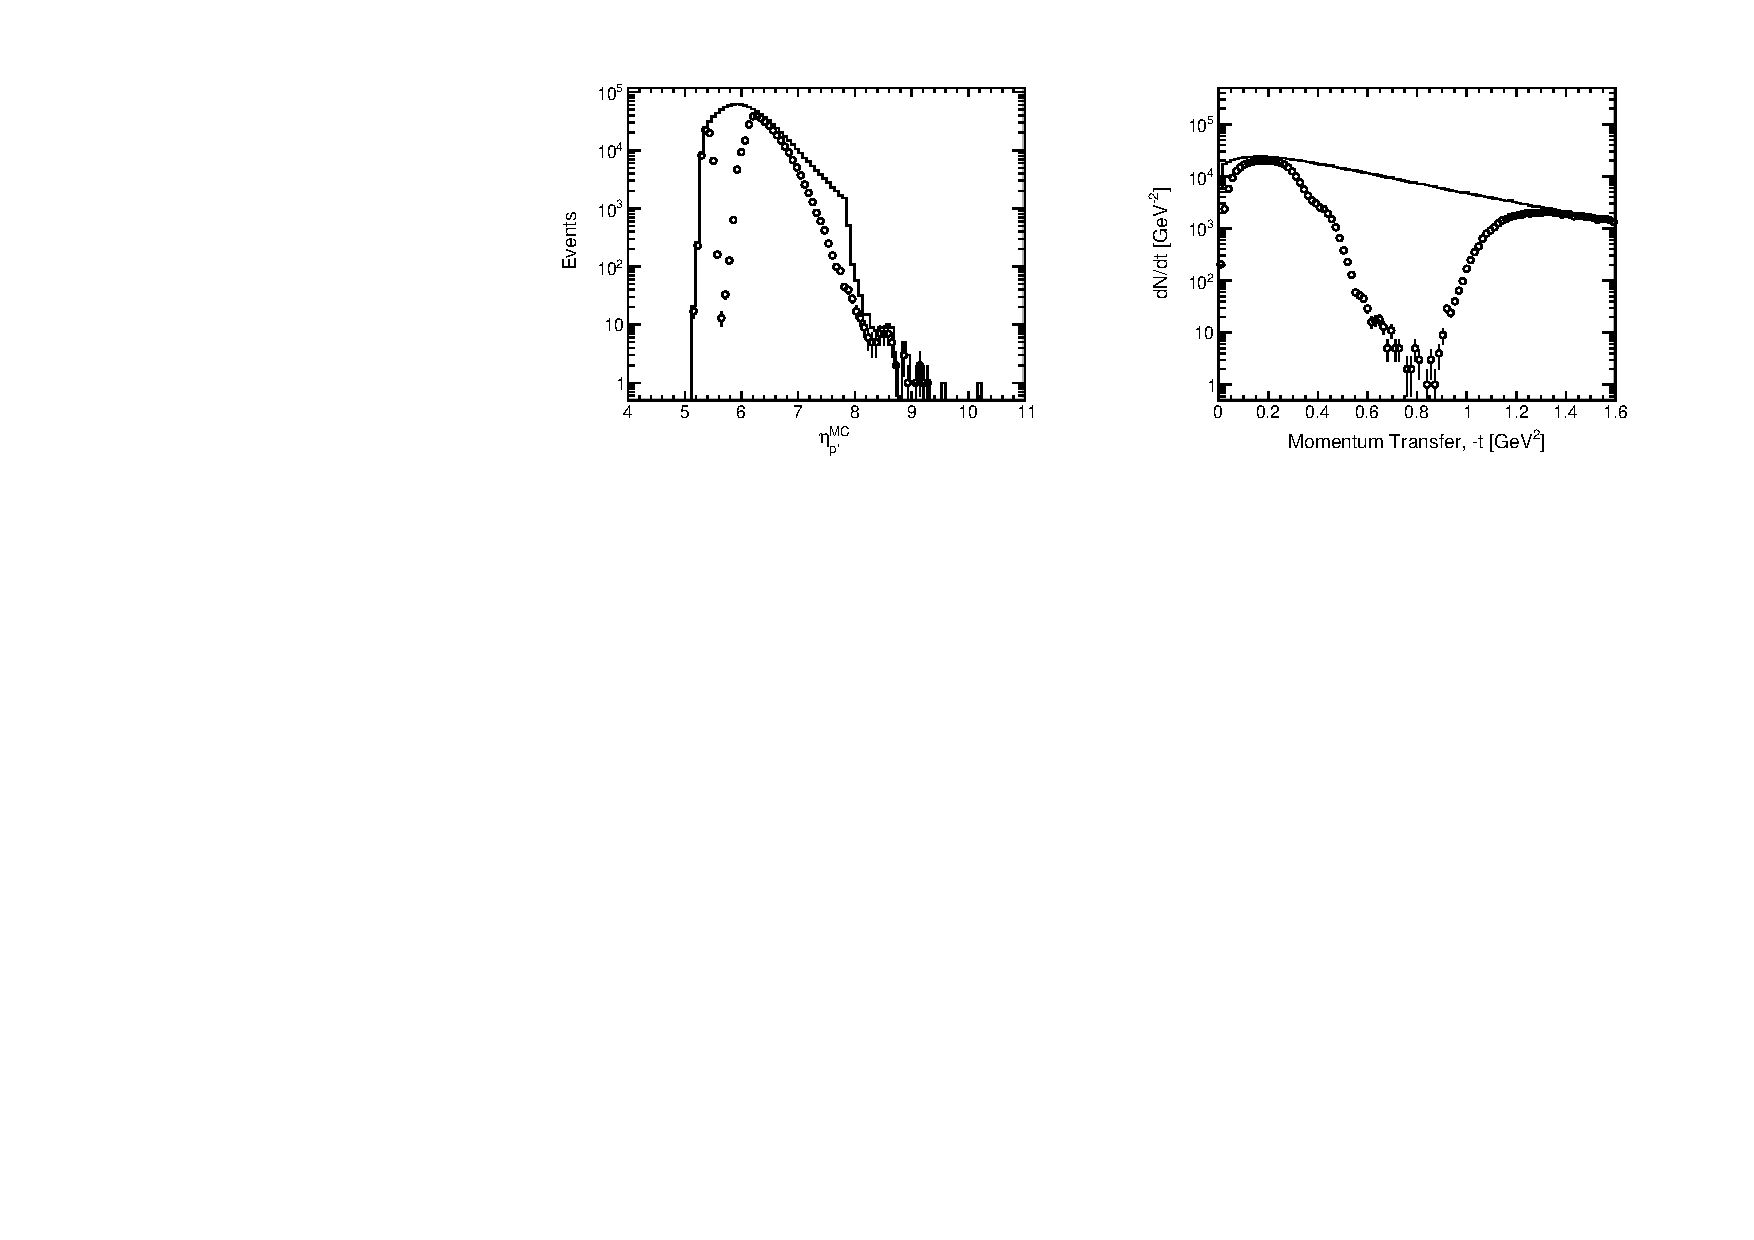
\includegraphics[width=0.75\textwidth]{Figures/proton_acc.pdf}
    \caption{(Left) Detector acceptance for the scattered proton as a function of pseudo-rapidity. (Right) Distribution of the squared momentum transfer, $t$, reconstructed from the accepted protons. The black solid line represents the true distribution, while the black open circles indicate the accepted true distribution within detector acceptance.}
\label{fig:protonacc}
\end{figure}

\begin{figure}[h]
    \centering
    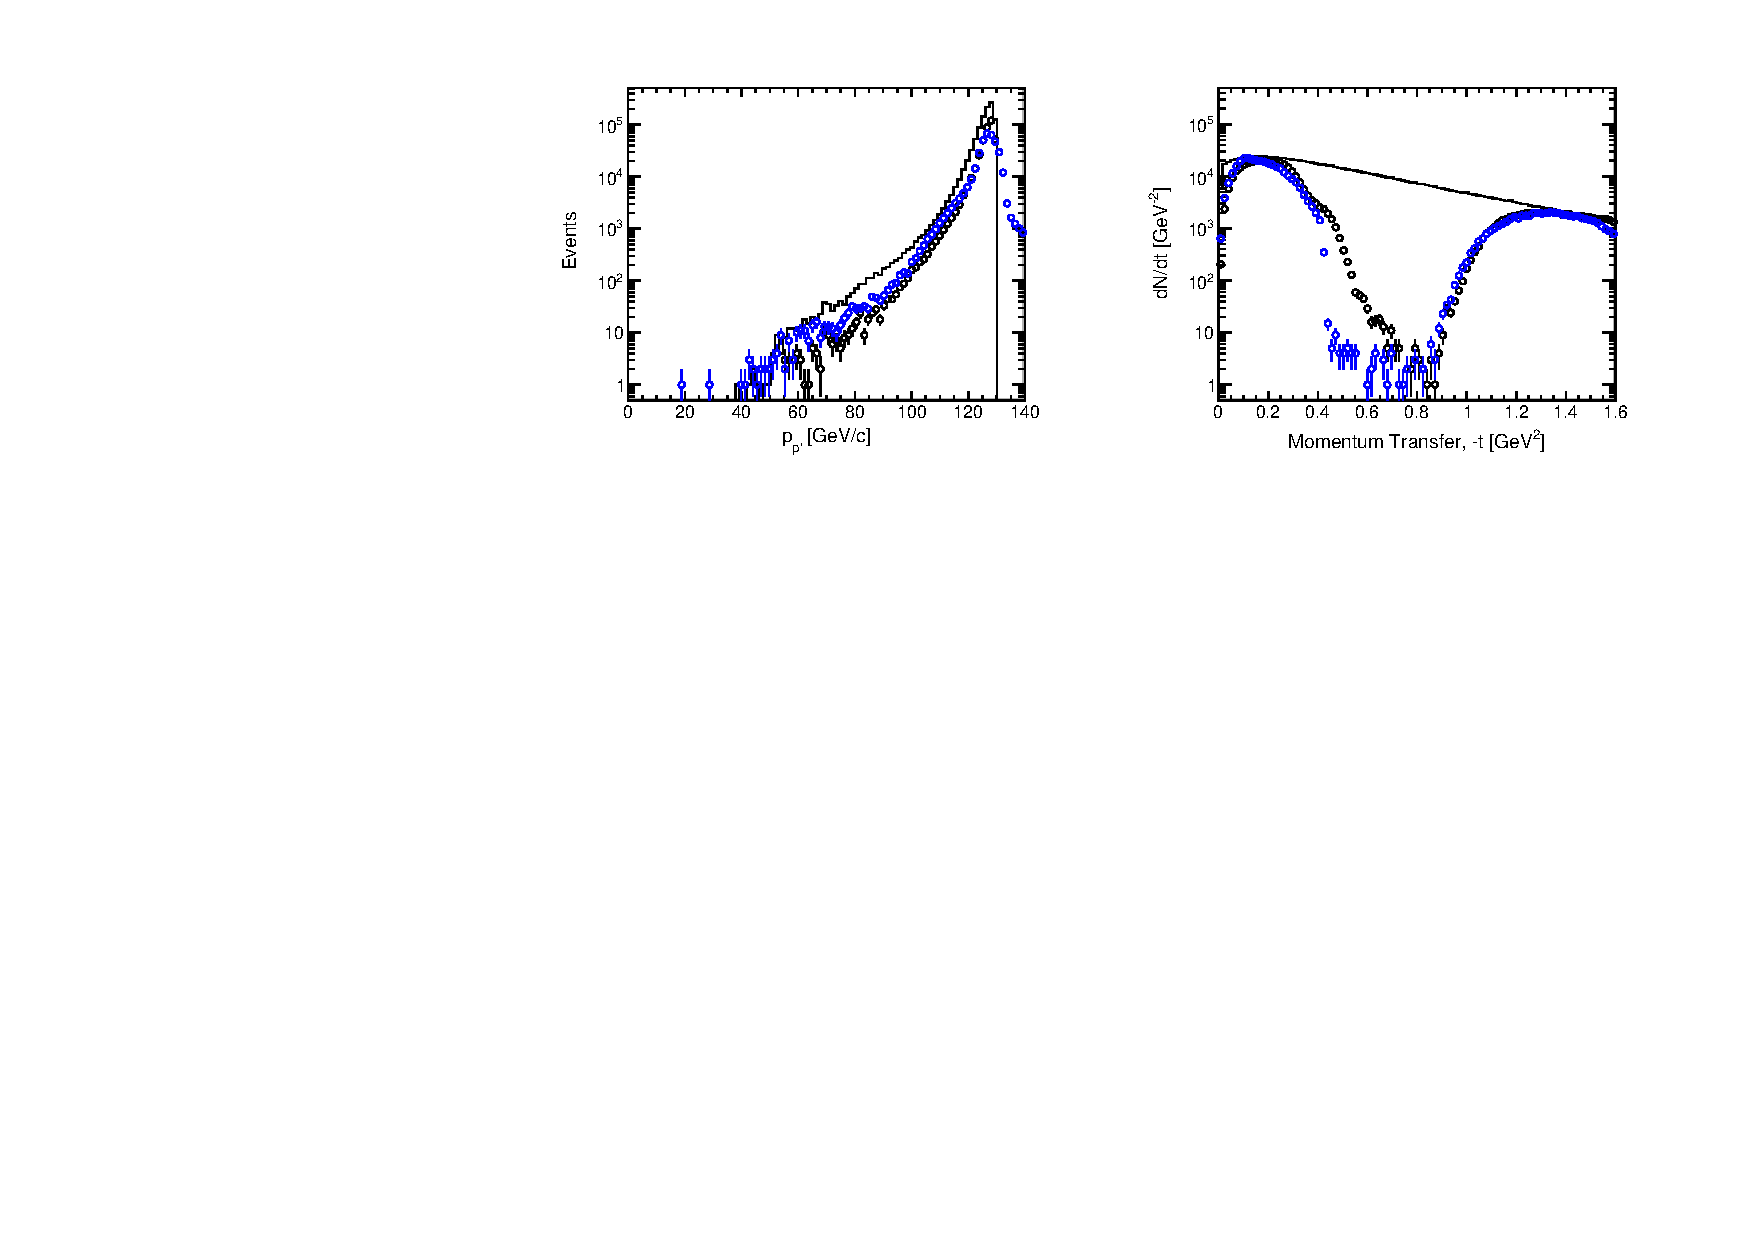
\includegraphics[width=0.75\textwidth]{Figures/proton_rec.pdf}
    \caption{(Left) Momentum distributions of the scattered proton. (Right) Distributions of the squared momentum transfer, $t$. The black solid line represents the true distribution, black open circles indicate the accepted true values within detector acceptance, and blue open circles show the reconstructed values.}
\label{fig:protonrec}
\end{figure}

\subsection{Neutral Pion}\label{subsec:NeutralPion}
% Acceptance and quality cut
Most of the decay photons from the produced $\pi^{0}$ are concentrated in the forward region. To reconstruct the $\pi^{0}$, the detector must identify both decay photons and accurately reconstruct their four-momenta. The left panel of Fig.~\ref{fig:pi0} shows the detector acceptance for neutral pion reconstruction, requiring both photons to be individually reconstructed. A noticeable loss of acceptance is observed in the mid-rapidity region, which is attributed to a non-optimized cluster splitting algorithm in the current ePIC reconstruction framework. This result suggests that there is significant potential to improve neutral pion acceptance through refinement of the clustering algorithms. The right panel of Fig.~\ref{fig:pi0} compares the momentum distributions of the true, acceptance-limited, and reconstructed neutral pions. To select well-reconstructed $\pi^{0}$ candidates, the invariant mass of the photon pair is required to lie within $\pm3\sigma$ of the nominal $\pi^{0}$ mass, as shown in Fig.~\ref{fig:pi0mass}.

\begin{figure}[ht]
    \centering
    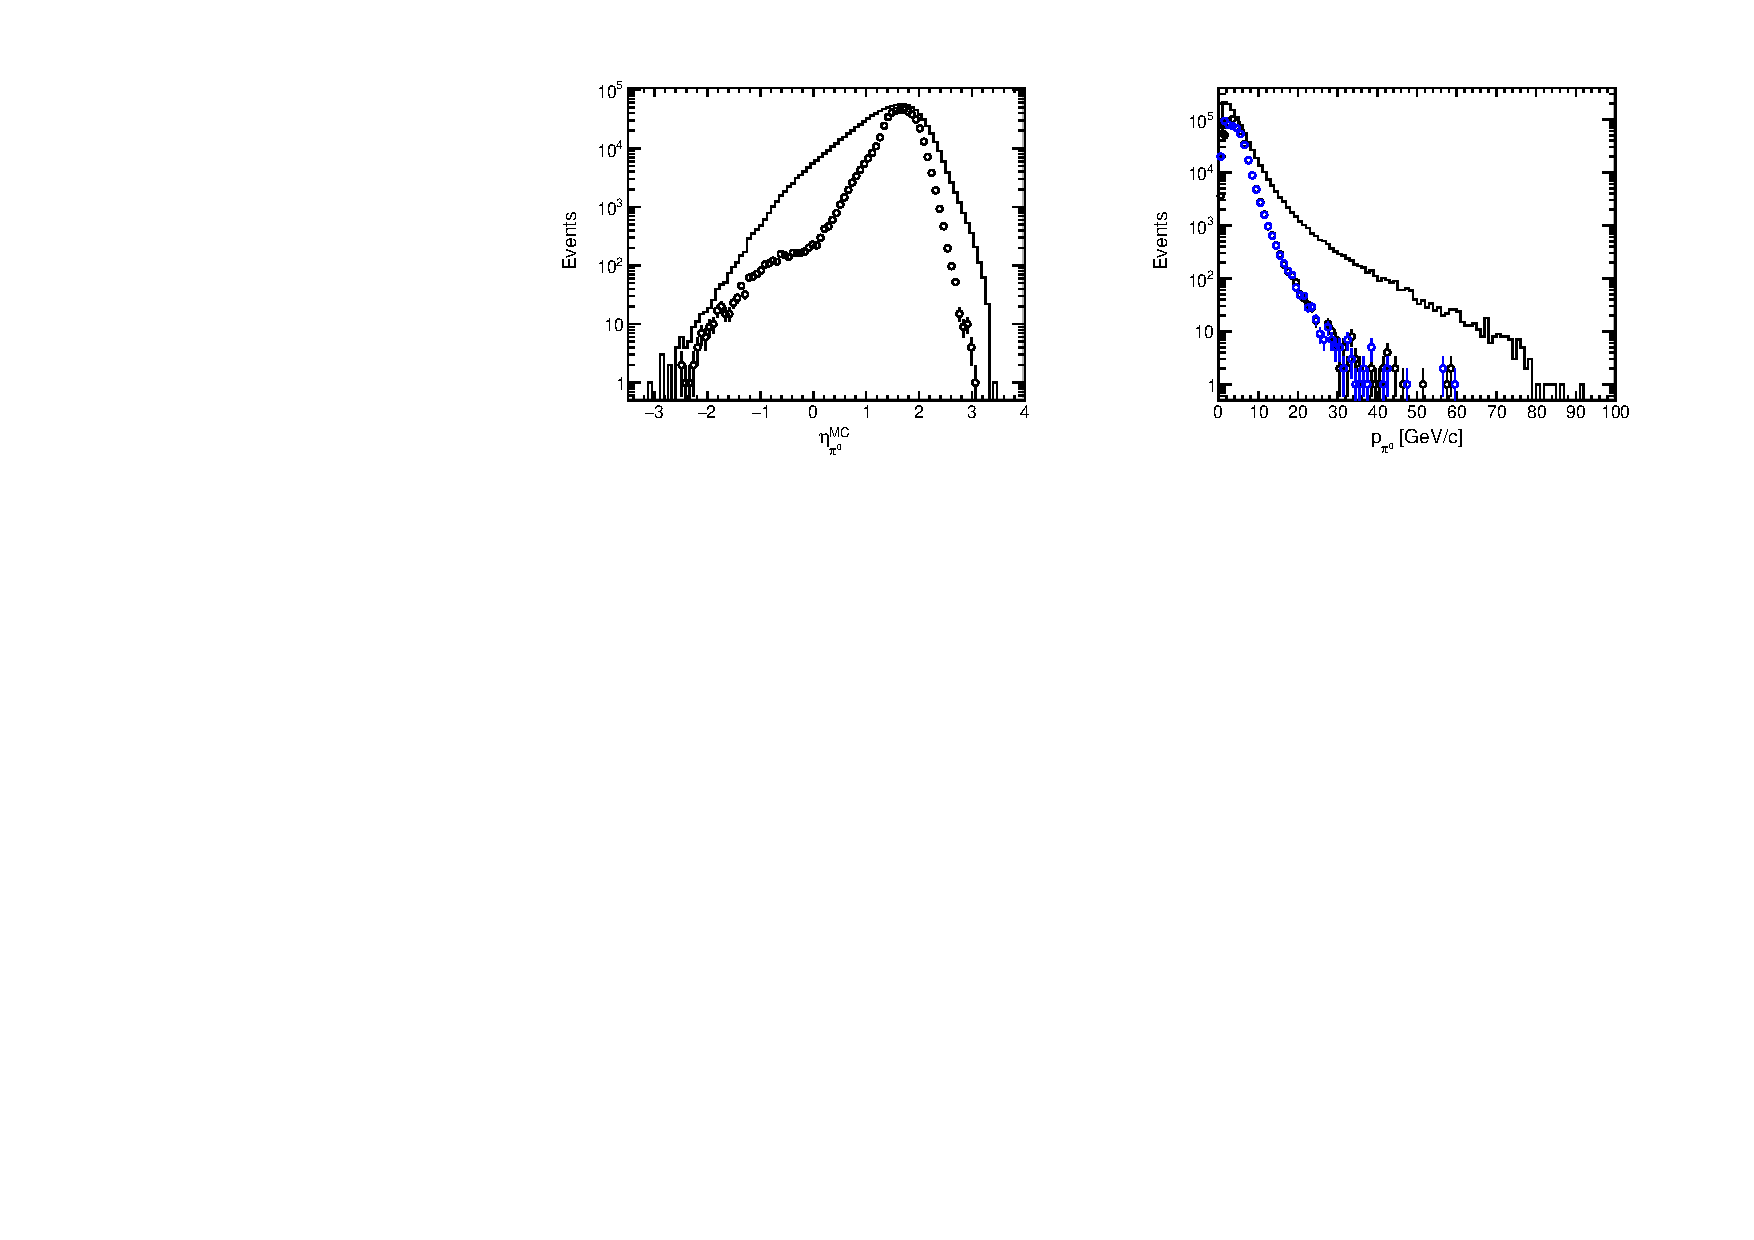
\includegraphics[width=0.75\textwidth]{Figures/pi0.pdf}
    \caption{(Left) Detector acceptance for $\pi^{0}$ as a function of pseudo-rapidity. (Right) Momentum distributions of the true $\pi^{0}$ (black solid line), accepted true values within detector acceptance (black open circles), and reconstructed values (blue open circles).}
\label{fig:pi0}
\end{figure}

\begin{figure}[ht]
    \centering
    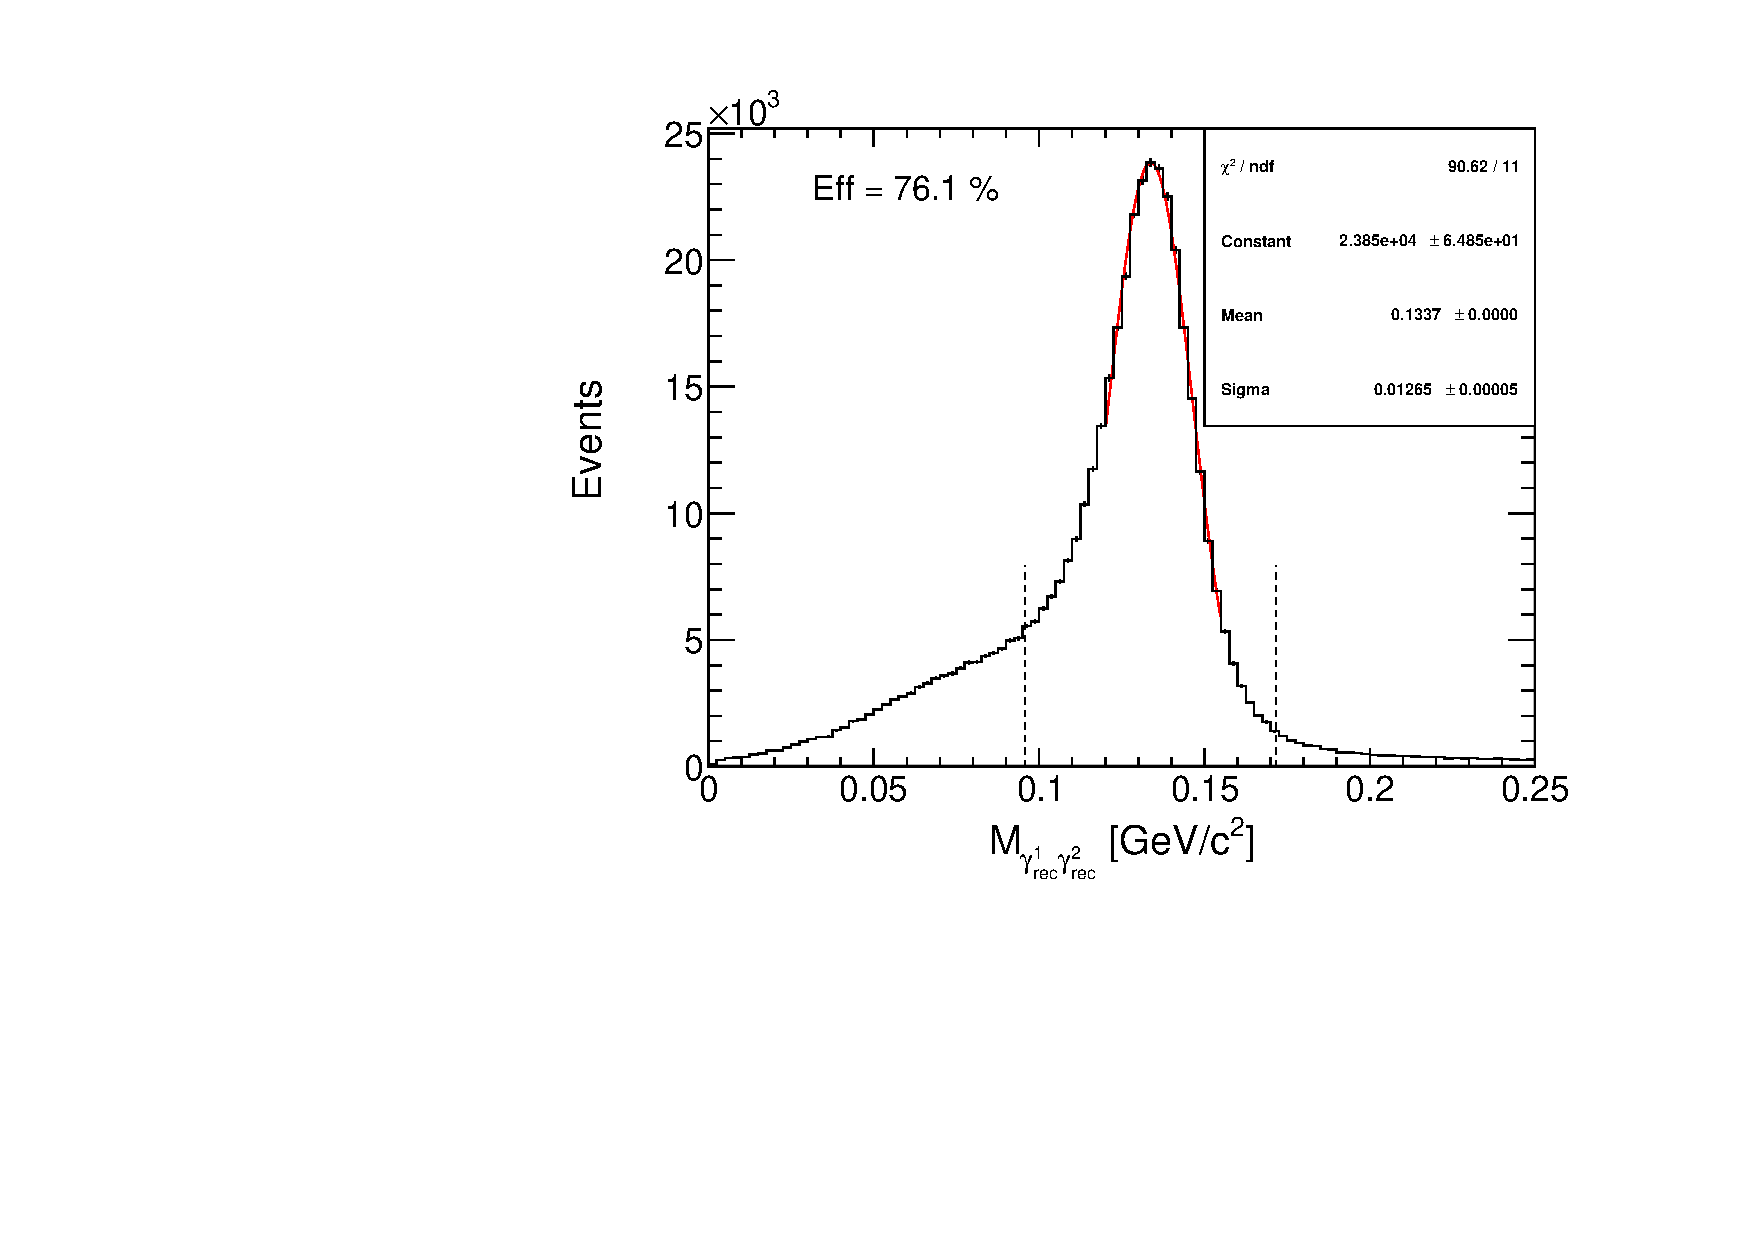
\includegraphics[width=0.4\textwidth]{Figures/pi0_mass.pdf}
    \caption{Invariant mass distribution of photon pairs from $\pi^{0}$ decays. Well-reconstructed $\pi^{0}$ candidates are selected by requiring the invariant mass to lie within $\pm3\sigma$ of the nominal $\pi^{0}$ mass.}
\label{fig:pi0mass}
\end{figure}

\subsection{Analysis Code}\label{subsec:Analysis_Code}
The analysis code is currently under development and is located at:
\begin{verbatim}
/gpfs02/eic/jkim/DVpi0P/scripts/WIP_updated.C
\end{verbatim}

\section{Background Contribution to DVCS}\label{sec:Background}
In the EIC Yellow Report, the minimum energy threshold for the forward electromagnetic calorimeter (EMCal) was set to 100MeV. At the request of the calorimeter group, a study was performed to evaluate the impact of increasing these thresholds to 200MeV in the pseudorapidity range $1.4 < \eta < 3.0$, and to 400~MeV in the range $3.0 < \eta < 3.5$. To assess the impact of these raised energy thresholds in the forward region, DV$\pi^{0}$P and DVCS event samples were generated, and a simplified study was conducted at the generator level. The effects were evaluated in terms of $\pi^{0}$ reconstruction efficiency and the resulting background contribution to DVCS measurements.

Fig.~\ref{fig:pi0_and_dvcs} shows the kinematic distributions of the two decay photons from $\pi^{0}$ in DV$\pi^{0}$P events and the single photon from DVCS events. The $\pi^{0}$ decay photons are predominantly produced in the forward region, while the DVCS photon is primarily distributed in the mid-rapidity region.

Regarding $\pi^{0}$ reconstruction efficiency, increasing the EMCal energy threshold from 100~MeV to 200~MeV in the range $1.4 < \eta < 3.0$ results in a modest overall impact, as shown in Fig.~\ref{fig:pi0_threshold_ratio}. The reduction in efficiency is primarily observed for low-momentum $\pi^{0}$s, where the efficiency drops by approximately 10~\%. High-momentum $\pi^{0}$s are less affected due to their more energetic decay photons. Although low-momentum $\pi^{0}$s dominate the cross-section, the total loss in reconstruction efficiency is partially offset by the preserved detection of higher-energy decay products. In the range $3.0 < \eta < 3.5$, increasing the threshold to 400~MeV has negligible effect, as $\pi^{0}$s in this region are typically highly boosted and their decay photons are well above the new threshold.

To quantify the background contribution to DVCS measurements, Fig.~\ref{fig:gamma_dist} compares photon momentum distributions from DV$\pi^{0}$P and DVCS events. The left panel corresponds to the 100~MeV threshold, and the right to the 200~MeV case. The DVCS histogram (blue solid line) is scaled to match the integrated luminosity of the DV$\pi^{0}$P sample (black solid line). The black open circles represent DV$\pi^{0}$P events where one decay photon is undetected due to threshold cuts, potentially mimicking a DVCS event.

To estimate the background contribution, we integrate the distribution of these single-photon events (where one photon is missed and the other is within detector acceptance) and compare it to the DVCS distribution. In the pseudo-rapidity range $1.4 < \eta < 3.0$, the background contribution is below 1~\% at the 100~MeV threshold and approximately doubles when the threshold is raised to 200~MeV. In the $3.0 < \eta < 3.5$ range, the background remains negligible, even with the increased threshold.

\begin{figure}[h]
    \centering
    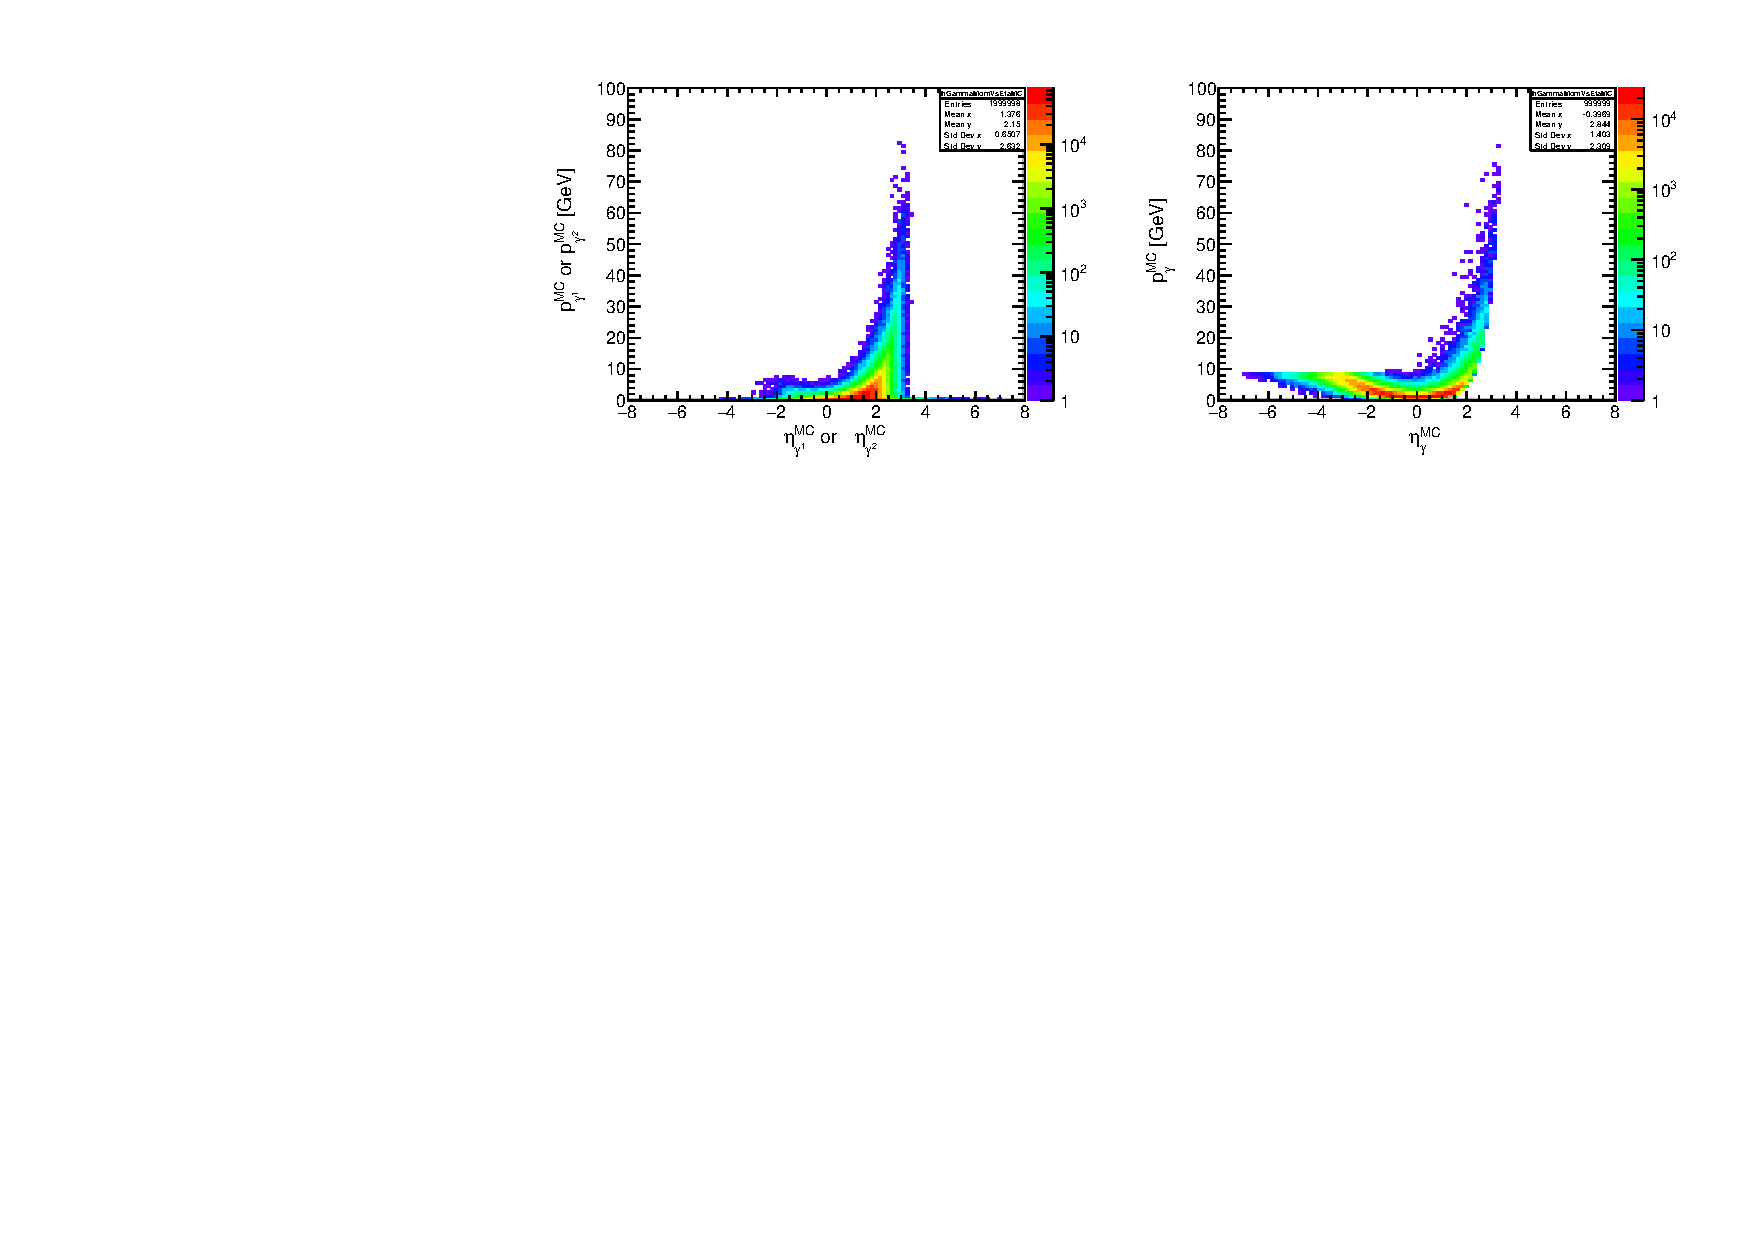
\includegraphics[width=0.75\textwidth]{Figures/Pi0GammaDVCSGamma.pdf}
    \caption{Kinematic distributions of the two decay photons from $\pi^{0}$ in DV$\pi^{0}$P events (left) and the single photon from DVCS events (right).}
\label{fig:pi0_and_dvcs}
\end{figure}

\begin{figure}[h]
    \centering
    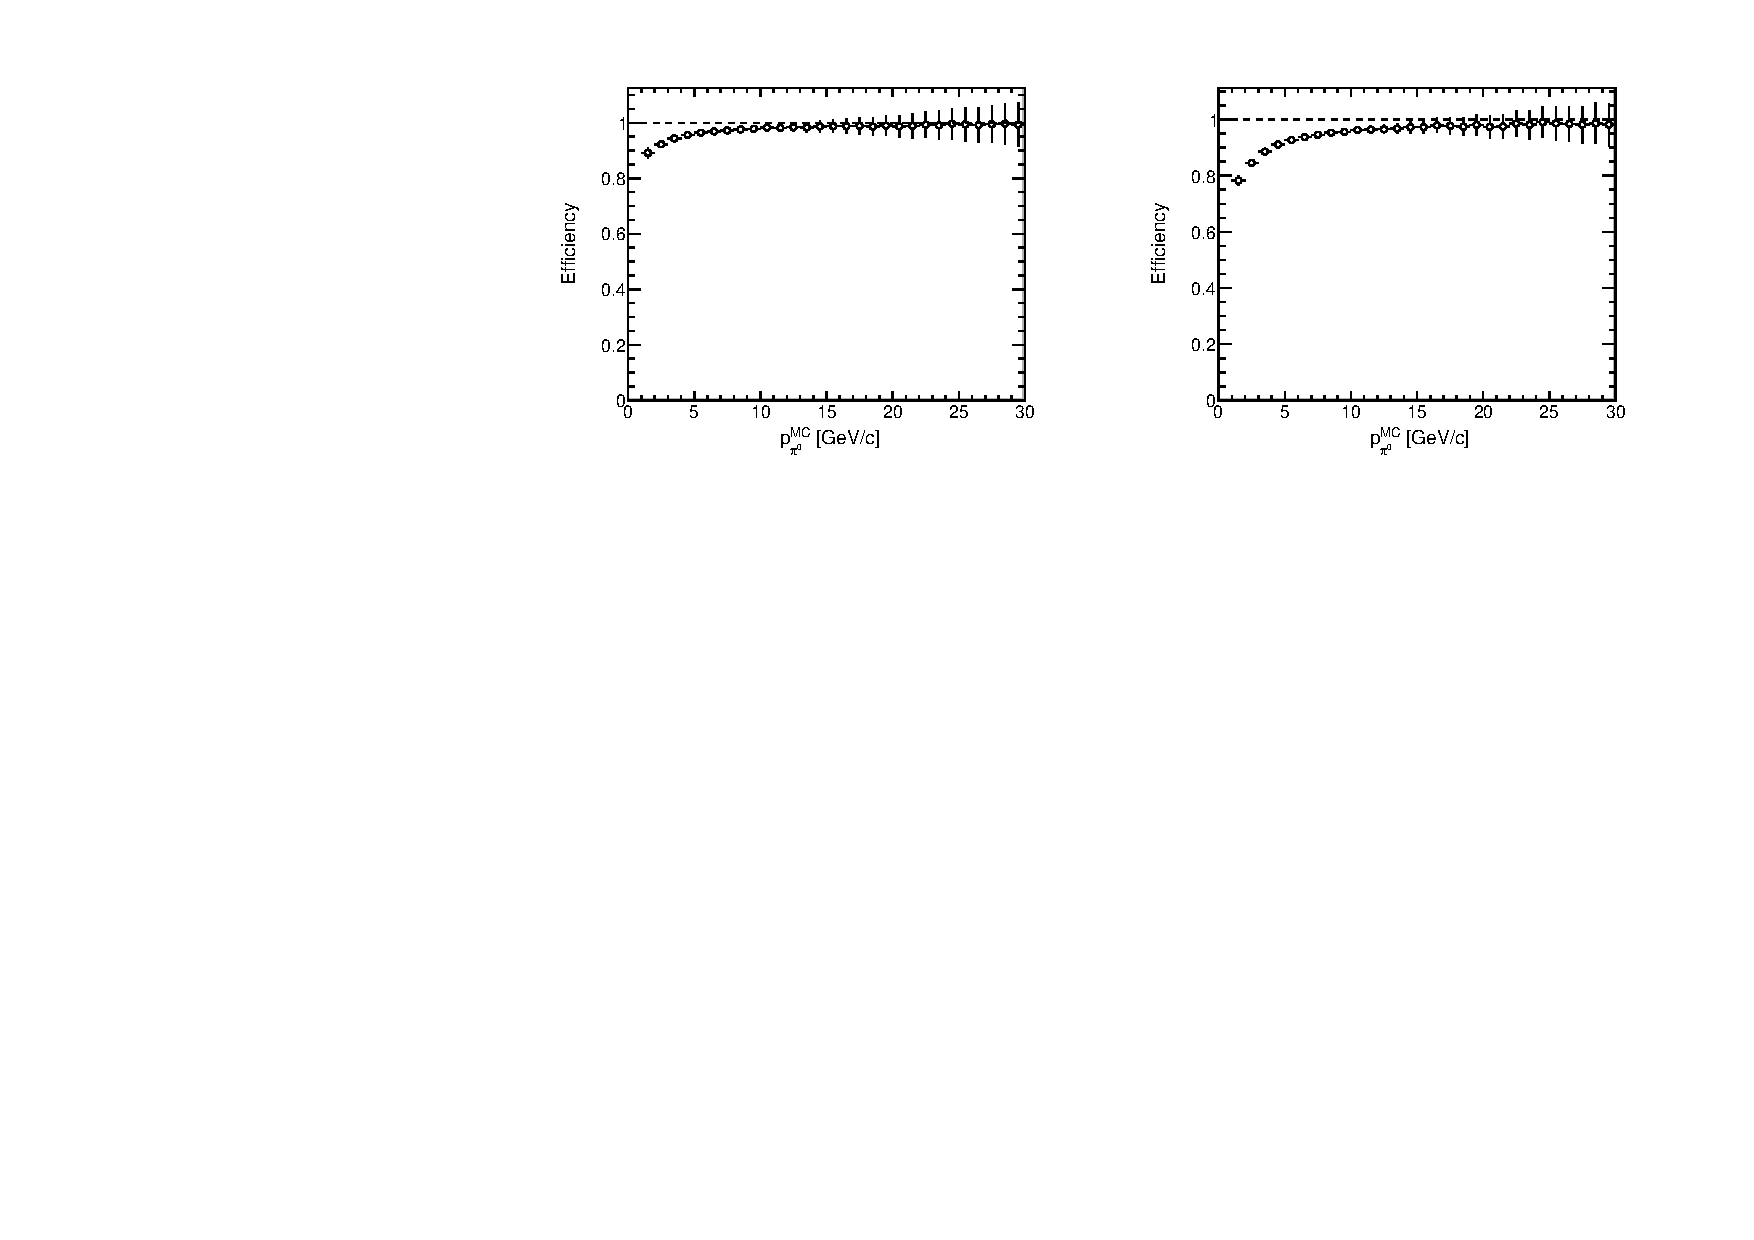
\includegraphics[width=0.75\textwidth]{Figures/hPi0ThresholdRatio.pdf}
    \caption{$\pi^{0}$ reconstruction efficiency as a function of momentum at minimal energy threshold 100~MeV (left) and 200~MeV (right) in the pseudo-rapidity range $1.4 < \eta < 3.0$.}
\label{fig:pi0_threshold_ratio}
\end{figure}

\begin{figure}[h]
    \centering
    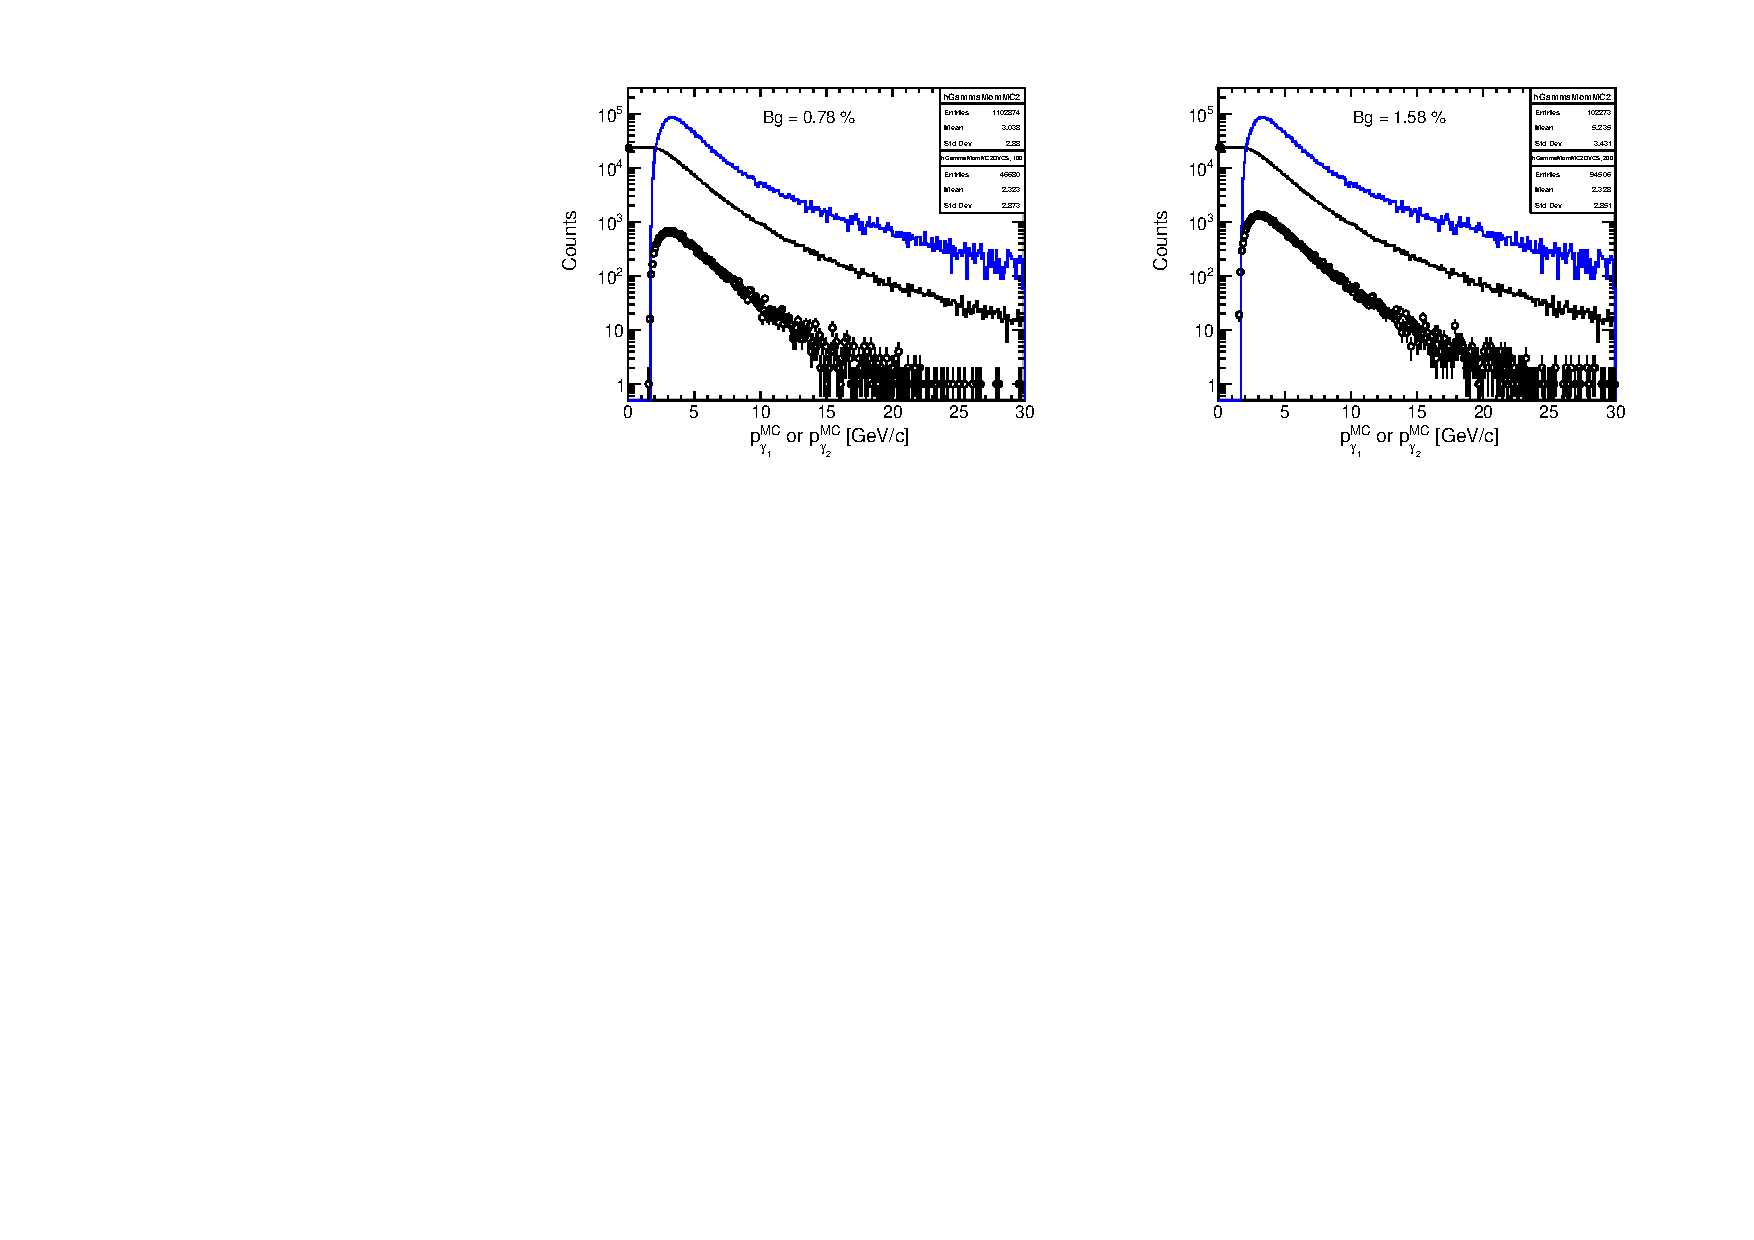
\includegraphics[width=0.75\textwidth]{Figures/hGammasMomMC2DVCS.pdf}
    \caption{Photon momentum distributions from DV$\pi^{0}$P and DVCS events at minimal energy threshold 100~MeV (left) and 200~MeV (right) in the pseudo-rapidity range $1.4 < \eta < 3.0$. The DVCS histogram (blue solid line) is scaled to match the integrated luminosity of the DV$\pi^{0}$P sample (black solid line). The black open circles represent DV$\pi^{0}$P events where one decay photon is undetected due to threshold cuts, potentially mimicking a DVCS event.}
\label{fig:gamma_dist}
\end{figure}

\pagebreak
\section{Results and Discussion}\label{sec:Results_Discuss}
% t distribution
[To Do] The distribution of the squared momentum transfer, $t$, will be shown after applying quality cuts on the reconstructed scattered proton.

\begin{figure}[ht]
    \centering
    \includegraphics[width=0.2\textwidth]{Figures/t_distribution_corrected.pdf}
    \caption{[placeholder] Differential cross-section for momentum transfer $t$.}
\label{fig:tdist}
\end{figure}

% phi distribution
To perform a feasibility study of the longitudinal single-target spin asymmetry, the $\phi$-distribution of the reconstructed $\pi^{0}$ was obtained, integrated over $t$, $x$, and $Q^{2}$. The resulting distribution is shown in Fig.~\ref{fig:phidist}. It has been corrected for detector acceptance, efficiency effects, and the crossing angle, while beam effects remain uncorrected. A fit using a $\sin(2\phi)$ functional form was applied to extract the amplitude of the asymmetry.

The analysis includes exclusivity cuts, requiring: (1) a well-identified scattered electron, selected using the $E/p$ criterion; (2) a well-reconstructed $\pi^{0}$, selected via the invariant mass window cut; and (3) full reconstruction of all final-state particles. The current DV$\pi^{0}$P sample is unpolarized, and, as expected, the extracted asymmetry amplitude is consistent with zero within 1$\sigma$ uncertainty.

The next step is to analyze a polarized proton DV$\pi^{0}$P sample in order to compare asymmetry amplitudes and assess the sensitivity of the measurement.

\begin{figure}[ht]
    \centering
    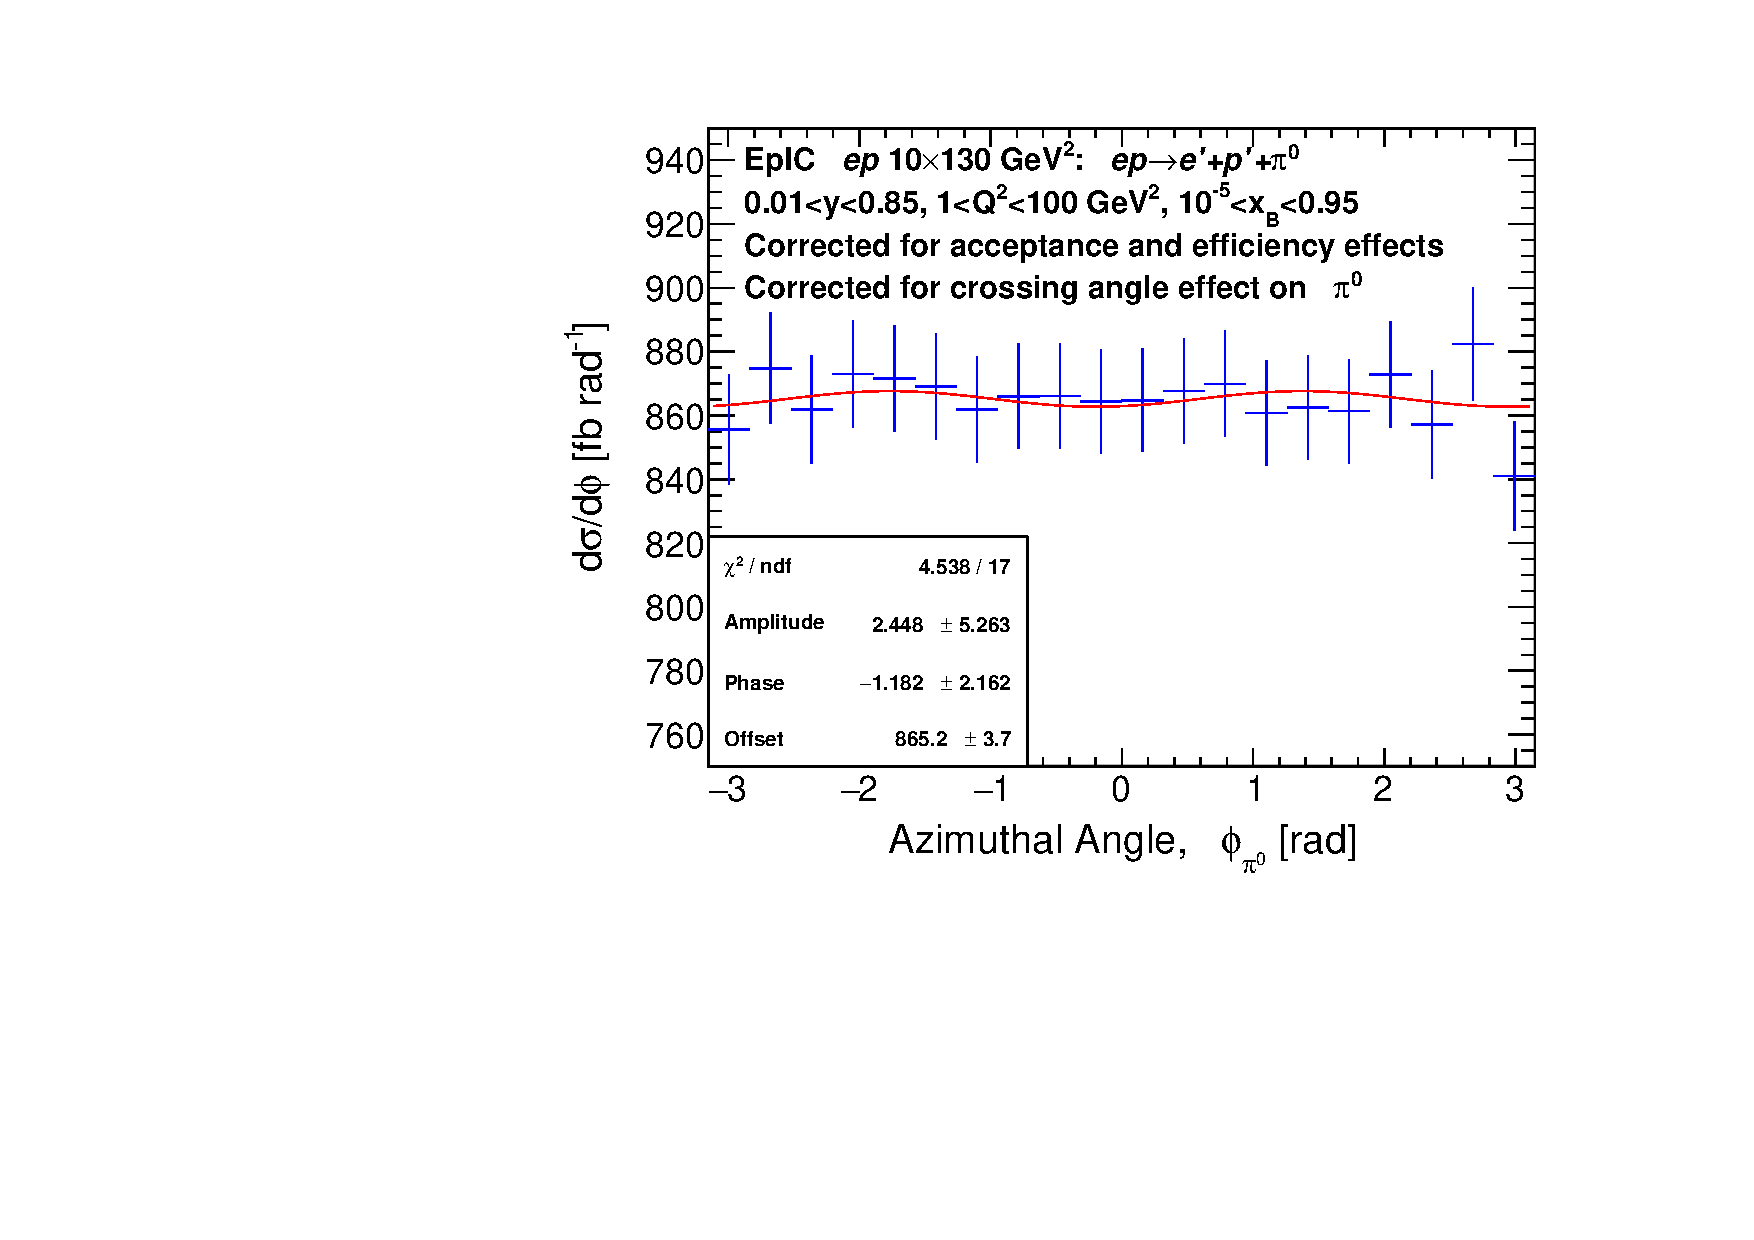
\includegraphics[width=0.5\textwidth]{Figures/phi_distribution_corrected_fit.pdf}
    \caption{The $\phi$-distribution of the reconstructed $\pi^{0}$ integrated over $t$, $x$, and $Q^{2}$. It has been corrected for detector acceptance, efficiency effects, and the crossing angle, while beam effects remain uncorrected. A fit using a $\sin(2\phi)$ functional form was applied.}
\label{fig:phidist}
\end{figure}

% discussion

%\pagebreak
\appendix
\section{Appendix}
Material you wish to include in an appendix. 

\bibliographystyle{elsarticle-num} 
\bibliography{bibliography.bib}

\end{document}